\documentclass[oneside,12pt]{book}

% Package dependencies
\usepackage{geometry}
\usepackage{lipsum}
\geometry{left=32mm, right=30mm, bottom=25mm, top=25mm}
\usepackage{amsmath , amsthm , amssymb}
\usepackage{float}
\usepackage{graphicx}
\usepackage{hyperref}
%\usepackage[]{apacite}
%\usepackage[nosectionbib,numberedbib]{apacite}
%\usepackage[natbibapa,nosectionbib,numberedbib]{apacite}
\usepackage[natbibapa]{apacite}

\usepackage{scrextend}
\usepackage{blindtext}
\usepackage{fancyhdr}
\usepackage{multicol}
\usepackage{csquotes}
\usepackage{bm}
\usepackage{subcaption}
\usepackage{tocbibind}
\usepackage{pdfpages}
\usepackage[toc,page]{appendix}
\usepackage{wrapfig}
\usepackage{colortbl}
\usepackage{multirow}
\usepackage{caption}
\captionsetup{font=small,labelfont=small}
\usepackage{titlesec}
\usepackage{listings}



\lstset{
  basicstyle=\ttfamily,
  columns=fullflexible,
  frame=single,
  breaklines=true,
  postbreak=\mbox{\textcolor{red}{$\hookrightarrow$}\space},
}
\setcounter{secnumdepth}{3}

% document formatting
\addtokomafont{labelinglabel}{\sffamily}
\setlength{\columnsep}{1cm}
\renewcommand{\baselinestretch}{1.5}
\newcommand{\myparagraph}[1]{\paragraph{#1}\mbox{}\\}


\begin{document}

% Title page
\begin{titlepage}
    \begin{center}
        \vspace*{1.5cm}
        
        \Huge
        \textbf{Analysis and Evaluation of Functionality of RAFT Consensus Algorithm in Internet of Things Domain}
        
        \vspace{0.5cm}
        \begin{figure}[H]
    	\centering
    	\hspace{7mm} \includegraphics[scale=0.5]{TU_logo}
        \end{figure}
        
        \vspace{1.5cm}
        
        \textbf{Bartosz Czapski}
        
        \vfill
       \large
        A dissertation submitted in partial fulfilment of the requirements of\\
	Dublin Institute of Technology for the degree of\\
	M.Sc. in Computing (Advanced Software Development)\\
       \vspace{0.5cm}
        \textbf{16/06/2022}
        \vspace{0.8cm}
 
    \end{center}
\end{titlepage}

% Define headers / footer style for the whole doc
\pagestyle{fancy}
\fancyhf{}
\fancyfoot[CE,CO]{\thepage}
\renewcommand{\headrulewidth}{0pt}



% APA style for referencing
\bibliographystyle{apacite}
\setlength{\bibleftmargin}{1cm}

% Roman numerals for the 'administrative' sections
\pagenumbering{Roman}

% Declaration page
\chapter*{Declaration}
\addcontentsline{toc}{chapter}{Declaration}
I certify that this dissertation which I now submit for examination for the award of
MSc in Computing (Stream), is entirely my own work and has not been taken
from the work of others save and to the extent that such work has been cited and
acknowledged within the text of my work.
\\
\\
This dissertation was prepared according to the regulations for postgraduate study of
the Dublin Institute of Technology and has not been submitted in whole or part for an
award in any other Institute or University.
\\
\\
The work reported on in this dissertation conforms to the principles and requirements
of the Institute’s guidelines for ethics in research.
\vfill
\noindent
\textit{\textbf{Signed:}}  \\
\begin{figure}[H]
    \raggedright
    
\includegraphics[width=0.3\textwidth]{LatexSkeleton/images/1655126301179.jpg}
\end{figure}
\noindent
\textit{\textbf{Date: June, 16, 2022}}
\vspace{0.8cm}

% Abstract
\chapter*{Abstract}
\addcontentsline{toc}{chapter}{Abstract}
\par In this thesis author examines significance of the leader-based consensus and its role in improving reliability of Internet of Things (IoT) devices seen as a broader self-organizing domain. Recent advances in the development of low-cost, single-board, high-performance interconnected devices able to receive and process data from multiple sources led to emergence of IoT which can be perceived as an invisible layer of cooperating sensors, working continuously in the background sensing, measuring, connecting and transmitting huge quantities of environmental data. Once collected, this data is perpetually transmitted either over the internet network or long range, low power, wireless platform (LoRa) to gateway nodes capable of storing, analyzing and processing it before passing events requiring careful consideration upstream, towards server-based data aggregation points. Due to amount of data collected and transmitted non-stop between the IoT nodes, implementation of IoT network presents a significant challenge. Attempts are being made to organize sensing devices, based usually on their location, into clusters that are capable of “intelligent” cooperation and working in unison. Among proposed solutions, achieving consensus between the associated devices motivated the research for this thesis. Building upon previous research, author decided to focus on two leader-based consensus algorithms, Paxos and RAFT, that are taking very similar approach to achieving distributed consensus and are well known and yet not fully implemented in the IoT universe. Although both algorithms are leader-based, Paxos requires all nodes within the cluster to exchange log entries while the election process is taking place. This allows for each node to participate in leadership election, but it increases complexity and network usage. On the contrary, RAFT algorithm requires node’s logs to be up to date to be considered for leader election process and it allows for highly efficient and reliable undertaking. During the research process, author investigated multiple recent works discussing distributed consensus in multi-agent systems (MAS) and attempted to implement RAFT and Paxos algorithms in IoT system to evaluate functionality of RAFT consensus algorithm and its advantages over Paxos algorithm in decreasing packet loss rate and latency in IoT network with LoRa.
\\
\vfill
\noindent
\textbf{Keywords:} \quad Raft, Paxos, consensus, IoT, LoRa

%Acknowledgements
\chapter*{Acknowledgments}
\addcontentsline{toc}{chapter}{Acknowledgments}
\par I would like to thank my supervisor, Dr. Bujar Raufi, for his ongoing support and advise
throughout this dissertation.\smallskip \newline 
I would also like to thank  my mother Halina, my father Krzysztof, and my sister Karolina, for their constant encouragement and support.\smallskip \newline
Finally, I would like to say a very special thank you to my girlfriend Federica for enormous support and patience. Without her encouragement and support this dissertation would never have been possible.

% Contents and lists
\newpage
\tableofcontents

\listoffigures

\listoftables

\lstlistoflistings

%\chapter*{List of Acronyms}
%\addcontentsline{toc}{chapter}{List of Acronyms}
%\begin{table}[H]
%  \centering
%    \begin{tabular}{ l l }
%    \textbf{ACRONYM1} & Meaning \\
%    \textbf{ACRONYM2} & Meaning \\ 
%    \end{tabular}
%\end{table}

\newpage

% Standard numbering starts from here
\pagenumbering{arabic}
\fancyhead[RE,LO]{\leftmark}
\renewcommand{\headrulewidth}{2pt}


% Start of core thesis content

%Introduction chapter
% ============================================================= %
\chapter{Introduction}
\par The goal of this master thesis is to carry out research on the leader-based distributed consensus algorithms, Paxos and Raft, and their role in achieving overall system reliability in the presence of a number of faulty processes or involving multiple unreliable nodes on the Internet of Things (IoT) network. IoT is a network of sensors and devices that can communicate and exchange data with each other through the Internet or long-range, low power, wireless platform (LoRa). As IoT importance increases annually since the first decade of 21st century, it is followed by the increase in the number of devices cooperating in the IoT network and an increase in the complexity of the communication infrastructure required to achieve flawless exchange of the data between the devices \citep{ismail2019introductory}. This constant connectivity necessitates a consensus mechanism that, once implemented, enables distinct nodes in an IoT network to agree on the authenticity and validity of transmitted data and increases the reliability of the distributed system \shortcites{8328431}\citep{8328431}. Therefore, this research paper’s main focus will be on implementing and maintaining distributed consensus among the IoT devices, and evaluating the performance of proposed algorithms in the presence of increased network latency due to faulty, or unreachable nodes. Additionally, we will attempt to compare the efficiency of both, Paxos and Raft, algorithms in decreasing packet loss rate and improving the system’s stability. 
\section{Background}
\par Nowadays distributed systems merge with the Internet of Things (IoT) creating a decentralized system of collaborating Smart Objects (SOs) which sense, store, and interpret information from the surrounding environment and act on their own, cooperate with each other exchange information with other kinds of IoT devices, or client nodes \shortcites{7488250}\citep{7488250}.\smallskip \newline 
The assumption that IoT network demonstrates properties comparable to distributed systems \citep{ICAR} opens the door to new solutions and implementations where Smart Objects cooperate together to achieve a common goal, akin to networked devices in the distributed system. Continuous attempts are made to design swarms of sensors that can encompass trillions of different devices capable of dynamically recruiting and disbanding additional resources \citep{6781658}, or to implement IoT across the urban areas creating SmartCity where, as \cite{JI2021101182} asserts, “centralized control method can neither reflect the spatial topology and physical constraints nor is it suitable for multi-sensor situations” leading, researchers involved, directly towards incorporating IoT into distributed systems paradigm \shortcites{XIAOYI2021106567}\citep{XIAOYI2021106567}.\smallskip \newline    
Although distributed systems seem like a natural approach to the design and implementation of IoT in real-life scenarios \shortcites{CHAMOSO2020323}\citep{CHAMOSO2020323}, an issue arises when orchestration and synchronization of devices are attempted \citep{AHMAD2020482}. Consensus is regarded as the primary problem which, once solved, will enable the implementation of a fault-tolerant distributed system \citep{MSR-TR-2005-33}. Consensus algorithms enable the collection of machines to cooperate as a coherent group, able to survive the failures of some of its members. This feature warrants consensus algorithms to play a key role in building reliable large-scale distributed systems \citep{10.5555/2643634.2643666} where the decisions are made by the conglomeration of devices acting as one system or service. Hence, distributed consensus algorithms, once adopted for IoT, will provide mechanism for balanced decision making on the edge nodes, and avoiding losing data from IoT devices in the presence of a number of malfunctioning devices by improving the robustness and reliability of the decision process \shortcites{6740862}\citep{6740862}.\smallskip \newline
Multiple authors recently focused on the idea of distributed consensus algorithms, their application in IoT domain \shortcites{BOF2017601,RAGHAV2020101291,whittaker2020matchmaker,ZHANG2020574,FORTINO202034}\citep{BOF2017601,RAGHAV2020101291,whittaker2020matchmaker,ZHANG2020574,FORTINO202034}, and implementation of self-organizing real-time systems architecture \shortcites{10.1007/978-3-030-30278-8_34,GUERRERO2019131,7488250}\citep{10.1007/978-3-030-30278-8_34,GUERRERO2019131,7488250}.


\section{Research Project/problem}
\par As mentioned by \shortcites{7058993}\cite{7058993}, “there are four major components in application systems with internet-of-things (IoT): sensors, communications, computation and service, where a large amount of data are acquired for ultra-big data analysis to discover the context information and knowledge behind signals. Therefore, it is not feasible to employ centralized solutions on cloud servers, especially in the case of IoT. Thanks to the advances of silicon technology, the cost of computation becomes lower, and it is possible to distribute computation on every node in IoT.” This approach leads to the integration and intertwining of both technologies, distributed computing and IoT and requires additional mechanisms focused on improving network throughput and reducing delays between the IoT nodes \citep{ImpRaft}.\smallskip \newline
A consensus algorithm is used to attain, in distributed and multi-agent systems, overall system reliability in the presence of a number of faulty processes or involving multiple unreliable nodes. When discussed in the context of IoT, a consensus algorithm is required to achieve fast event ordering, predictable delivery time and minimal packet loss rate in edge computing networks.\smallskip \newline
Current approaches to consensus between the nodes in IoT domain include modifying existing consensus algorithms: blockchain \shortcites{WANG2020101871,10.1007/978-3-030-30278-8_34}\citep{WANG2020101871,10.1007/978-3-030-30278-8_34}, cooperative game model \citep{GULATI2020102222}, proportional-integral-derivative (PID) \citep{SHI201873}, developing new algorithm \citep{8737532}, or using revised Paxos consensus algorithm \citep{10.5555/3324320.3324322,Cachin}.\smallskip \newline 
In this paper, we will research the feasibility of implementing Paxos and Raft consensus algorithms in IoT networks and assess their effectiveness in enabling fault-tolerant distributed IoT. The following sections will introduce particulars relevant to distributed IoT networks and review both algorithms in detail.
\subsection{Distributed System}
\par A distributed system is a collection of independent devices that can be scattered across different locations, yet able to cooperate with each other and share the computing power of the cluster to accomplish shared objectives.
\begin{figure}[H]
\centering
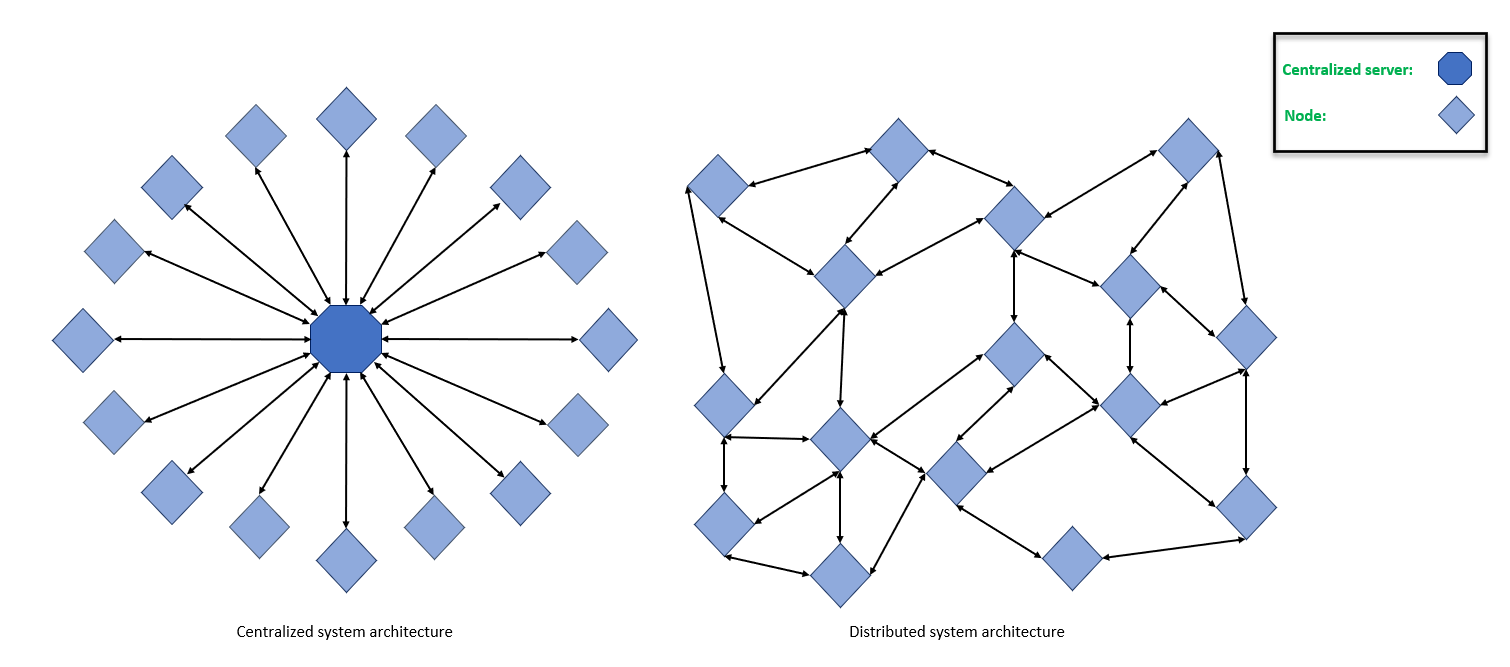
\includegraphics[width=1\textwidth]{LatexSkeleton/images/centralizedvsdist.PNG}
\caption{Centralized vs. Distributed system architecture}\shortcites{10.1007/978-981-13-8300-7_2}\citep{10.1007/978-981-13-8300-7_2}
\end{figure}
\noindent For all intents and purposes, distributed system performs as a one interface or service and will appear as a uniform to the client process or end-user. Below properties outline typical characteristics of the distributed system \shortcites{PUDER20067}\citep{PUDER20067}:
\begin{itemize}
  \item Scalability\smallskip \newline Additional processing nodes are easily added to the cluster to improve the computing efficiency of the system.
  \item Loosely coupled\smallskip \newline Nodes are communicating with each other using a standard protocol but have very little direct knowledge of each other.
  \item Concurrency\smallskip \newline Nodes that create distributed system run simultaneously. 
  \item Heterogeneity\smallskip \newline The nodes and components of a distributed system can be of different types and designs which does not affect its efficiency or scalability.
  \item Replication\smallskip \newline The distributed system implements information and messaging sharing, ensuring consistency between the nodes affecting in improved reliability and accessibility.
  \item Availability and fault-tolerance\smallskip \newline Node failure does not lead to a system failure; the remaining nodes will continue to operate and attempt to complete the system’s objectives.
\end{itemize}
\noindent The idea of distributed system translates directly to IoT domain \shortcites{7058993}\citep{7058993} and its characteristics align with IoT network.
\subsection{Byzantine vs non-byzantine distributed systems}
\par \shortcites{10.1145/357172.357176}\cite{10.1145/357172.357176} proposed a problem that describes an issue of communication and trust in distributed computing, the Byzantine Generals Problem. It shows how problematic is the achievement of a common objective when the identity and intentions of the collaborators are unknown and possibly hostile.  Subsequently, the Byzantine network became synonymous with the system where some of the collaborating nodes are malevolent and unreliable and non-Byzantine became synonymous with the network of trustworthy and reliable nodes.\smallskip \newline 
Both algorithms, Raft and Paxos described and explained further in this paper, are distributed consensus algorithms that are specifically developed for non-Byzantine systems and require modifications to operate in the Byzantine network.
\subsection{Replicated State Machine}
\par State machine replication (SMR) is a mechanism that is implemented to transform a cluster of unreliable hosts into a single fault-tolerant service that, for the purpose of client devices connecting to it, provides strong consistency and linearizability \citep{StateMachine}. Therefore, the correct implementation of SMR allows client machines to treat service as a single system and anticipate expected behaviour. Most importantly, replicated state machine stipulates that the state machine of each node in the distributed system receives exactly the same operations in the exact same order. This requirement can be guaranteed by achieving distributed consensus \shortcites{194954}\citep{194954}.

\begin{figure}[H]
\centering
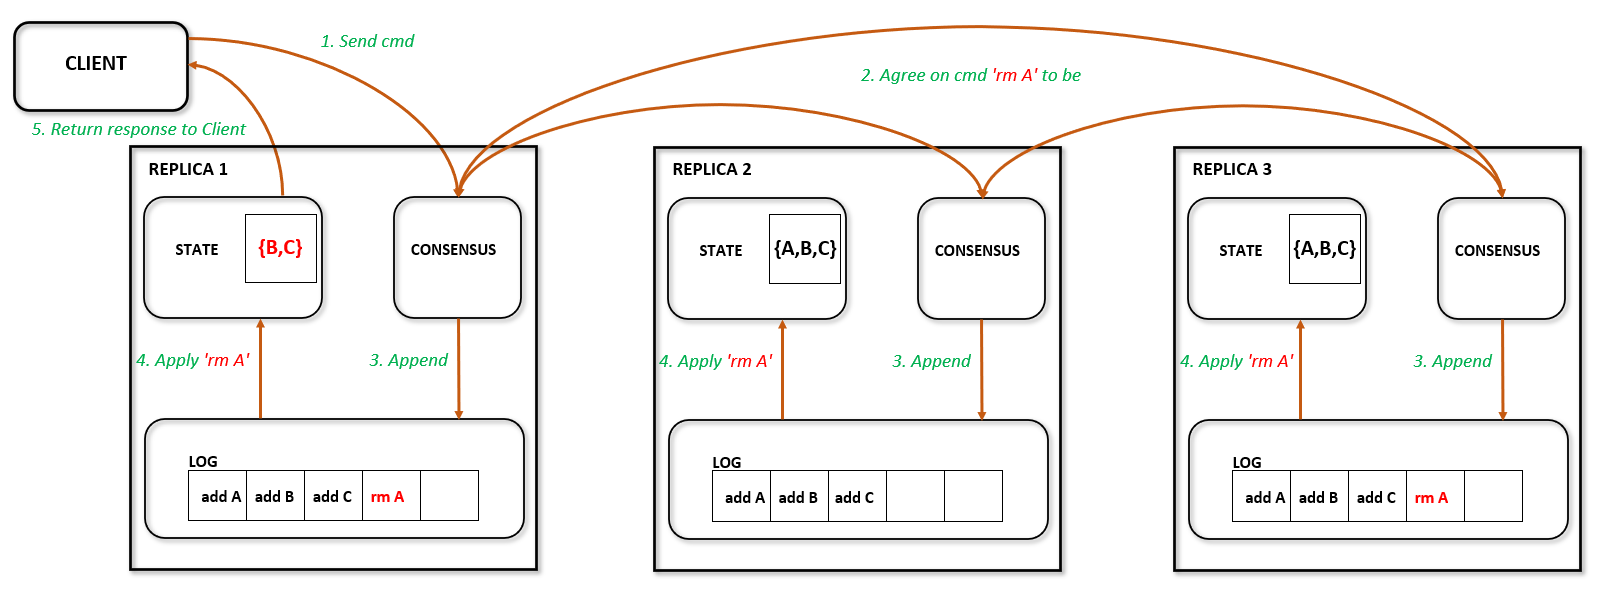
\includegraphics[width=1\textwidth]{LatexSkeleton/images/replicated.PNG}
\caption{Replicated State Machine }\citep{StateMachine}
\end{figure}

\subsection{Consensus}
\par \shortcites{6740862}\cite{6740862} classify IoT “as a network of networks, in which smart “things” are connected to the Internet via heterogeneous access networks and technologies (such as sensor networks, mobile networks, RFID, etc.) to provide services and applications” and similarly \cite{OROSTICA201915} perceive it as “a sparsely coupled, distributed system of interacting smart objects, or things.”\smallskip \newline
Both depictions of IoT imply that a certain level of autonomy is required for the devices forming an IoT network to operate and avoid failures. The sheer amount of the nodes coupled with a constant flow of the data require a mechanism that can ensure stability and optimal performance of the system. \smallskip \newline
One of the proposed solutions to the above problem is distributed consensus, which can be described as a mechanism that allows a group of nodes on an unreliable network to reach an agreement \citep{DistributedConsensus}. Consensus in distributed systems is necessary to achieve general system reliability in the face of multiple faulty nodes.
\subsection{Paxos}
\subsubsection{Introduction}
\par Paxos consensus algorithm was developed by Leslie Lamport in 1989 to solve the problem of fault-tolerant distributed systems, where collections of multiple separated devices can deterministically and safely agree on implementing certain actions under required conditions while guaranteeing the system’s consistency if the conditions cannot be satisfied \citep{LI2020247}. Often seen as an archetype of non-Byzantian consensus algorithms, Paxos is famous for being difficult to understand and hard to implement on distributed systems. This perception forced the author of the original paper to publish a series of explanatory articles where each step of the original algorithm was discussed and explained in plain English \citep{lamport1998the,lamport2001paxos,MSR-TR-2005-33}.
\subsubsection{Achieving Consensus}
\myparagraph{Roles}
Paxos perceives distributed system and its behaviour as a collection of roles, where each device can assume more than one role in the cluster. Each node participating in achieving consensus can accept and perform the roles below:

\begin{itemize}
  \item Client:\smallskip \newline The client is not a member of the distributed system. It issues a request to the cluster and expects a response. Paxos cluster is seen as a single coherent system to the client.
  \item Acceptor / Voter:\smallskip \newline Acceptor participates in the maintenance of fault-tolerant distributed storage in the cluster. Change to a state in a Paxos cluster cannot be committed until a quorum, a group of all acceptors, agree on it.
  \item Proposer:\smallskip \newline The proposer is a node that received a request from the client. It will attempt to persuade a quorum of acceptors to agree upon it.
  \item Leader:\smallskip \newline A Proposer who had a proposal accepted recently becomes a leader. Paxos requires that there is only one leader serving client requests. Only when the current leader fails, a new one selected and starts communicating with the client. 
  \item Learner:\smallskip \newline Learners are responsible for processing the request from the client, once the proposal was accepted, and sending the result back to the client.
\end{itemize}

\pagebreak

\myparagraph{Phases}
\begin{figure}[H]
\centering
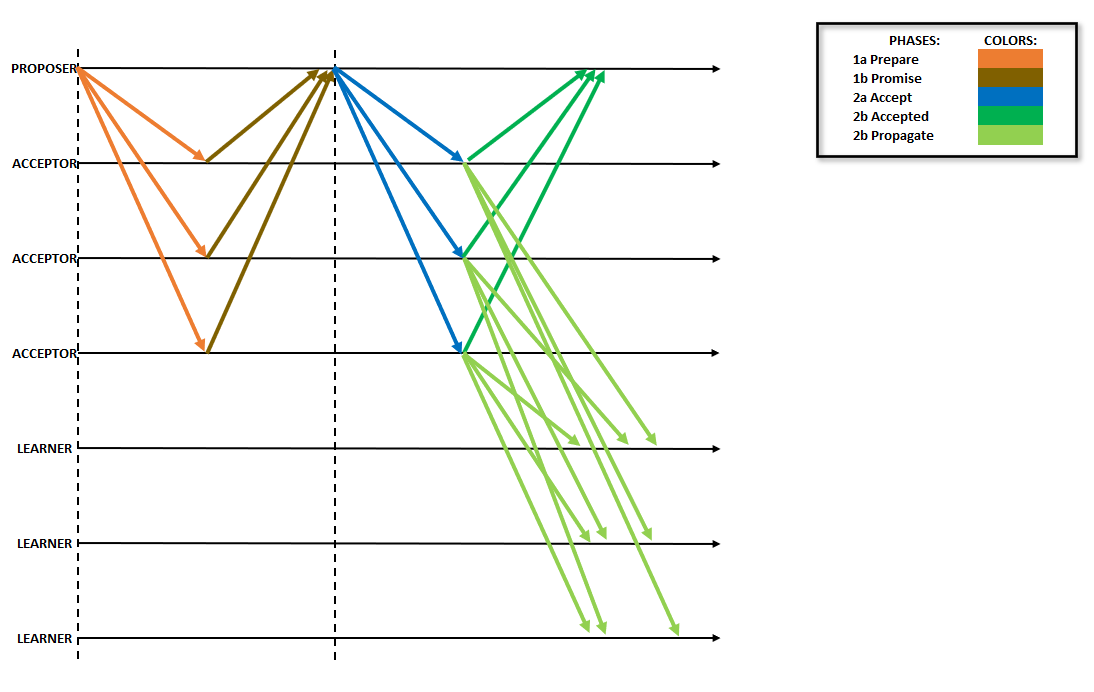
\includegraphics[width=1\textwidth]{LatexSkeleton/images/paxos_phases.PNG}
\caption{Paxos Phases}\citep{lamport2001paxos}
\end{figure}

\par Phase 1:
\begin{itemize}
  \item 1a Prepare:\smallskip \newline Whenever the proposer in a Paxos cluster receives a request from the client, it sends a proposal message to update the replicated state machine with the new client request to the quorum for acceptance. Proposal message, called prepare request, is in the form of \texttt{Prepare(n)} where n is autoincrementing identifier therefore each following prepare request from a given proposer will have a guaranteed unique n higher than the previous one.
  
  \item 1b Promise:\smallskip \newline Each of the acceptors in the quorum compares the n-value of the message to the previously accepted “Prepare” messages and if the newly received n-value of the “Prepare” message is higher, it sends the “Promise” message back to the proposer. If the Acceptor node accepted a different proposal message previously, it must then include the previous proposal n-value(m) and the corresponding value(v), in the “Promise” message returned to the Proposer (\texttt{Promise(n, (v, m)}), otherwise, if none were accepted previously it will be set to null (\texttt{Promise(n, null)}). This guarantees that the acceptor will not accept any other “Propose” messages with an n-value lower than currently accepted.
\end{itemize}
If the proposer receives promise messages from the majority of the quorum it attempts Phase 2 of the Paxos consensus algorithm.\smallskip \newline

Phase 2:
\begin{itemize}
  \item 2a Accept:\smallskip \newline Once promises from the majority of acceptors are received, the proposer node has to set its own v-value. As acceptors must return any v-values previously accepted, the proposer will set its current “Propose” v-value to the value of the highest proposal number in any of the “Promises” received. Only when all promise messages are empty (\texttt{null}), the proposer can set its own v-value. Subsequently, accept message request is sent to the quorum of acceptors (\texttt{Accept(n,v)}).
  
  \item 2b Accepted:\smallskip \newline Upon receiving \texttt{Accept(n,v)} message, acceptors have to accept it unless they issued promise message with n-value higher than accept n-value. \texttt{Accepted(n,v)} message is sent to proposer node and learner nodes, and the new value becomes consensus and it's committed to the replicated state machine.
\end{itemize}
Once the majority of acceptors agrees on it, request is processed by the learner nodes, and the result is returned via proposer node to the client.

\pagebreak
\subsubsection{Electing leader}
\par Paxos does not provide a leader election mechanism. It is advised to implement an algorithm responsible for choosing the leader, as Paxos might reach livelock when there is no progress made by the algorithm due to concurrent proposals from multiple nodes \citep{10.1145/3380787.3393681}. There are multiple solutions to leader election, one being the Bully algorithm proposed by \cite{UnderstandingPaxos}, where “a node that starts an election sends its server ID to all of its peers. If it gets a response from any peer with a higher ID, it will not be the leader. If all responses have lower IDs than it becomes the leader. If a node receives an election message from a node with a lower-numbered ID, then the node starts its own election. Eventually, the node with the highest ID will be the winner.” It is important to note that Paxos’ design is fault-tolerant and leader election is not required for achieving consensus, as proposals can be made by any of the Proposer nodes.

\subsubsection{Failure prevention and recovery}
Whenever a failure occurs in the cluster and the leader is unavailable, Paxos consensus algorithm assures that the nodes are won’t stop sending proposals leading to the election of a new leader with the highest proposal’s n-value. To resolve this issue Paxos might require multiple rounds of proposal messages sent back and forth leading to very inefficient network utilization and algorithmic efficiency.

\subsubsection{Conclusion}
Paxos algorithm attempted to solve consensus problems in non-byzantine distributed systems. It achieves its goal by strictly following two essential properties, as described by \cite{lamport2001paxos}:

\begin{itemize}
  \item “No value ever reaches consensus without first being proposed and having its proposal accepted.”
  
  \item “No two distinct values ever reach consensus at the same time.”
\end{itemize}

\subsection{Raft}
\subsubsection{Introduction}
\par Raft distributed consensus algorithm is the result of the work of \cite{10.5555/2643634.2643666} who attempted to create a leader-based consensus protocol that would be able to achieve similar performance and fault tolerance as Paxos but requires less complexity during implementation. Raft’s design reflects the need for better understandability of distributed consensus and the steps required to achieve it. Paxos algorithm, often viewed as a predecessor of Raft and a gold standard for distributed consensus algorithms, presents a significant challenge for developers and system designers during system analysis and implementation phases \citep{10.5555/2643634.2643666}. Authors of the Raft protocol listed Paxos complexity and convolution as the main reasons for developing Raft.

\subsubsection{Achieving consensus}
Raft algorithm achieves consensus via an elected leader. Raft cluster is built of exactly one leader and multiple followers, and a node in a cluster can be either leader or follower (in case of unavailability of the leader, the follower becomes a candidate and undergoes the election process).  Although all nodes in the distributed system can receive requests from the external clients, only the leader node is allowed to exchange data with the client and all requests received by follower nodes are forwarded to the leader.
\begin{figure}[H]
\centering
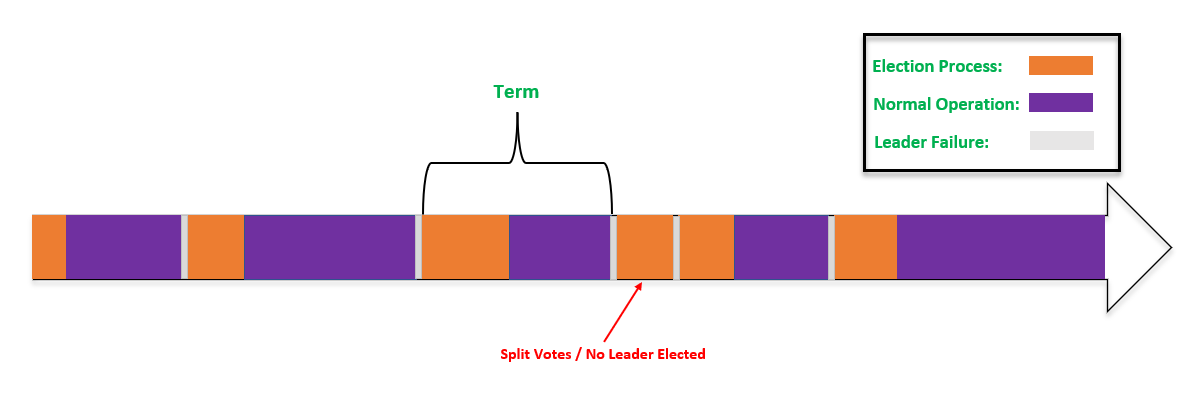
\includegraphics[width=1\textwidth]{LatexSkeleton/images/raft_terms.PNG}
\caption{Raft Terms}\citep{10.5555/2643634.2643666}
\end{figure}
\noindent Term is a time unit used by Raft that can be of random length, and each of the terms is given a consecutive number. Each leader is chosen during the election process that marks the start of a new term. If, during the election, no leader is chosen Raft will restart the election process effectively starting a new term. This step guarantees that during the term there is only one leader in the cluster. It is important to note that terms are used in Raft protocol context as a distributed system’s logical clock and, as each node stores the current term number, it allows to detect outdated data on the participating nodes. As mentioned by \cite{10.5555/2643634.2643666}, “current terms are exchanged whenever servers communicate; if one server’s current term is smaller than the others, then it updates its current term to the larger value. If a candidate or leader discovers that its term is out of date, it immediately reverts to the follower state. If a server receives a request with a stale term number, it rejects the request.”


\subsubsection{Electing leader}
Raft utilizes heartbeat messages to implement the leader - followers relationship, where each of the followers expects heartbeat from the leader within the so-called election timeout frame. Each node in the cluster starts as a follower and expects a valid heartbeat message from the leader node. The election process starts when a message is not received within the time limit, otherwise, the election timeout is reset \citep{10.5555/2643634.2643666}.

\begin{figure}[H]
\centering
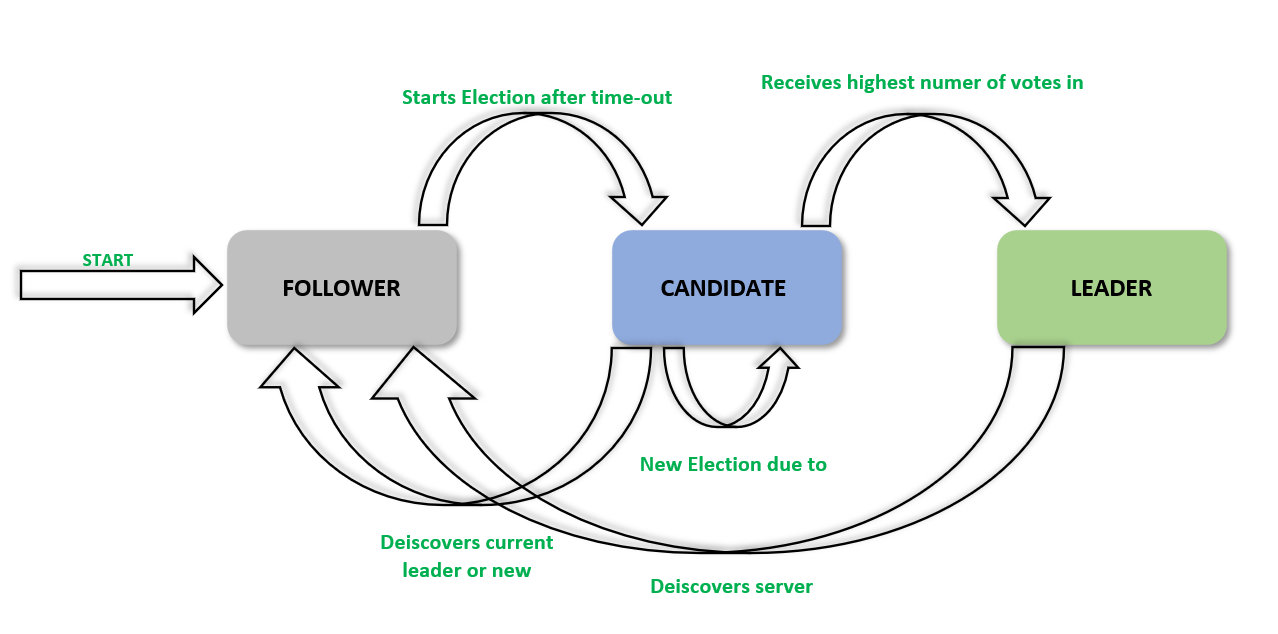
\includegraphics[width=1\textwidth]{LatexSkeleton/images/raft_election.PNG}
\caption{Raft election process }\citep{10.5555/2643634.2643666}
\end{figure}

\noindent The election starts with a follower transiting to the candidate by incrementing its current term number. This is followed by a \texttt{RequestVote} heartbeat message and voting for itself. All follower nodes in the cluster are expected to participate in the election process in parallel, and they remain in the candidate state until one of them wins the election or previously established time passes without selecting the leader. Immediately after the leader is elected, it broadcasts the heartbeat message to the entire cluster which stops the election process.

\subsubsection{Log replication}
The leader node’s main responsibility is to communicate with the clients and fulfilling their requests. Every one of those requests is stored within the leader’s logs and once the leader updates its log with a new entry, it will send an \texttt{AppendEntries} heartbeat message to the followers and expects that this command will be replicated within the cluster. The result is then returned to the originator after followers confirm the append request and the message is applied to the leader’s state machine. It is the leader’s sole responsibility to update the state machine with new entries and every commit is stored along the term number ensuring its validity. In their paper, \cite{10.5555/2643634.2643666} indicate that Raft is capable of achieving a high level of consistency among the cluster’s logs by implementing the properties below:

\begin{itemize}
  \item “If two entries in different logs have the same index and term, then they store the same command.”
  
  \item “If two entries in different logs have the same index and term, then the logs are identical in all preceding entries.”
\end{itemize}

\subsubsection{Failure prevention and recovery}
Raft consensus protocol implements a failure prevention and recovery mechanism where, in case of the inconsistency between the leader’s and follower’s logs, the follower will replicate the leader’s entries by overwriting its own. The process of checking and replicating logs is embedded within \texttt{AppendEntries} messages and it does not require extra steps from the leader node, as it is automatically executed from the moment of a successful election.

\subsubsection{Conclusion}
Raft has an advantage over the other consensus algorithms, noticeably Paxos, that its understandability is greatly improved \citep{UCAM-CL-TR-857} and its design is optimized for systems design and architecture \citep{10.5555/2643634.2643666}. Authors of the Raft protocol focused on strong leadership and the leader’s decisive role in achieving distributed consensus. As of the date of writing this thesis, there is unsubstantial work on the Raft algorithm being used in distributed IoT architecture for achieving consensus among the edge nodes.

\subsection{Paxos vs Raft}
Both previously described consensus protocols are sharing similar properties and follow similar assumptions, i.e.:

\begin{itemize}
  \item One of the nodes in the cluster is the leader, who accepts requests from clients and sends log entries to the follower nodes.
  
  \item A new entry is committed and once accepted, the state machine is replicated in the cluster.
  
   \item A new leader is elected by the majority as soon as the previous leader is unavailable (requires additional implementation in Paxos algorithm).
\end{itemize}
Most importantly, Paxos and Raft satisfy by design requirement mentioned by \cite{10.1145/3380787.3393681}:

\begin{itemize}
  \item “Theorem3.1 (StateMachine Safety). If a server has applied a log entry at a given index to its state machine, no other server will ever apply a different log entry for the same index.
  
  \item There is at most one leader per term and a leader will not overwrite its own log so we can prove this by proving the following:\smallskip \newline
  Theorem 3.2 (Leader Completeness). If an operation op is committed at index i by a leader in term t then all leaders of terms $>$ t will also have operation op at index i.”
  
\end{itemize}

\begin{table}[H]
  \centering
  \label{tbl:Summary of the differences between Paxos and Raft}
  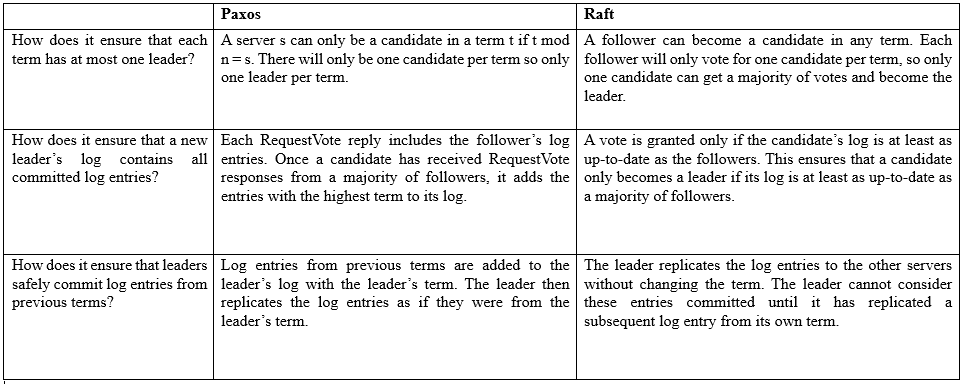
\includegraphics[width=1\textwidth]{LatexSkeleton/images/raft_paxos_tbl.PNG}
  \caption{Summary of the differences between Paxos and Raft}
\end{table}



\section{Research Objectives}
The aim of this research is to implement, analyse and evaluate the performance of the Raft consensus algorithm on IoT networks in the presence of multiple node failures. As current research on the topic of consensus problems in IoT domain does not discuss, nor benchmark Raft, the author will attempt to provide performance measurements (latency and packet loss rate) in the presence of different numbers of malfunctioning devices. Additionally, the results of the above experiment will be compared against the results of Paxos algorithm and IoT network without algorithm implemented.
Following research objectives would facilitate the achievement of this aim:

\begin{itemize}
  \item Constructing IoT network of three, five and seven Raspberry PI 3 Model A+ single-board computer and DockerPi Sensor Hub Development Board (EP-0106) and one Raspberry Pi 3 B acting as an IoT gateway.
  
  \item Implementing Paxos and Raft consensus algorithms on IoT network.
  
   \item Evaluating performance of proposed IoT network in the presence of multiple node failures when:
   \begin{itemize}
   
        \item No consensus algorithm is implemented
  
        \item Paxos consensus algorithm is implemented
  
        \item Raft consensus algorithm is implemented
   
   \end{itemize}
   \item Analysing the results of the experiments and providing recommendations for consensus implementation in IoT networks. 
   
\end{itemize}
We will conduct an experiment where original (non-existent) data will be collected, and different consensus algorithms will be compared to confirm if the implementation of Raft consensus algorithm in IoT network can decrease packet loss rate and latency of the network in the presence of malfunctioning edge nodes when compared to Paxos consensus algorithm?\smallskip \newline
Quantitative (numerical) data from the experiment will be collected and analysed to provide a definitive result. Exhaustive answers will be provided by comparing quantitative data that will test and confirm an existing theory.

\section{Research Methodologies}
Following on different classification of research methodology \citep{WOHLIN2021106678}, author recognizes that this research can be characterized in four distinct ways:

\begin{itemize}
  \item By type: Primary research\smallskip \newline
    An experiment will be conducted where original (non-existent) data will be collected. The generation of the data will begin as soon as the IoT nodes are powered up and the sensors start transmitting environmental information over the LoRa to gateway node. During the control experiment Packet Loss Rate (PLR) and latency between the client and edge note, and packet rate will be measured in IoT network. A control experiment will be repeated for each consensus algorithm, Paxos and Raft.
  
  \item By objective: Quantitative research\smallskip \newline
    Quantitative (numerical) data from the experiment will be collected and analysed and provide a definitive result. T-test with paired samples will be used to statistically compare performances of consensus algorithms during both experiments with different conditions. 
  
   \item By form: Empirical research\smallskip \newline
    The answers will be provided by comparing quantitative data by statistically comparing all data collected during control experiment algorithms performances during research experiments.
   
   \item By reasoning: Deductive research\smallskip \newline
    Author will test and confirm an existing theory. Proposed hypotheses H1, H2, H3 and H4 will be accepted independently based on the results achieved. Confirmation of hypotheses will confirm the research question.
\end{itemize}
\section{Scope and Limitations}
The scope of this research is to implement Paxos and Raft consensus algorithms on the IoT network where we will measure the algorithms’ performance. As consensus algorithms are necessary for achieving reliability in the distributed network \citep{10.1145/357172.357176}, this thesis will attempt to determine if the implementation of consensus algorithms in IoT networks will decrease Packet Loss Rate and latency on the network in the presence of malfunctioning nodes. Additionally, the findings will help to determine if the Raft consensus algorithm achieves better results than Paxos in attaining reliability on IoT networks.\smallskip \newline
Important limitation of this research is the size of the IoT networks used in the experiments. We will create and execute experiments based on three types of IoT networks, i.e., 3-node, 5-node and 7-node networks. The aforementioned network sizes were chosen based on the Paxos and Raft requirement of a minimum number of nodes to achieve consensus \texttt{(N/2 + 1)}. Although either of the proposed networks should achieve consensus in the presence of faulty nodes, this experiment would benefit greatly if the implementation of both algorithms was carried out on a larger scale, both from a network size and geographical location point of view. Additionally, Paxos is allegedly a difficult algorithm to implement on a distributed system \citep{10.5555/2643634.2643666} which might impede the course of this research.

\section{Document Outline}
This research paper is divided into five chapters where each chapter clearly defines the scope and objectives.\smallskip \newline 
In Chapter One, an outline of the research problem is provided together with an environment where the experiments will be conducted. Additionally, Chapter One describes research objectives and research methodologies utilized and clearly defines scope and limitations of this study.\smallskip \newline  
Chapter Two presents the most up to date research on the topic of consensus in distributed systems and delivers comprehensive review of the work carried out in the consensus field with clearly defined research gaps.\smallskip \newline
Chapter Three describes the design of the experiments carried out to answer the research question.\smallskip \newline
Chapter Four contains the detailed description of each experiment conducted. It also provides the technical specifications of the IoT networks implemented and the snippets of the code with its functionality described in the detail.\smallskip \newline   
Chapter Five discusses results of experiments performed.\smallskip \newline
Chapter Six is the final chapter that concludes the research work presented in this master thesis.\smallskip \newline

% Literature review chapter
% ============================================================= %
\chapter{Review of existing literature}

\section{Introduction}
This section provides an overview of the existing research and literature review that attempts to solve consensus conundrums in the IoT domain.\smallskip \newline
When mentioning consensus algorithms in the context of IoT, we have to clarify that their task is to enable the collection of machines to cooperate as a coherent group, able to survive the failures of some of its members. This feature warrants consensus algorithms to play a key role in building reliable large-scale distributed systems \citep{10.5555/2643634.2643666}.\smallskip \newline
As presented further in this section, multiple authors recently focused on the idea of distributed consensus algorithms, their application in IoT domain \citep{BOF2017601,RAGHAV2020101291,whittaker2020matchmaker,ZHANG2020574,FORTINO202034}, and implementation of self-organizing real-time systems architecture \citep{10.1007/978-3-030-30278-8_34,GUERRERO2019131,7372286}.\smallskip \newline 
Distributed consensus algorithms, when adopted for IoT, provide a mechanism for balanced decision making on the edge nodes and avoiding losing data from IoT devices in the presence of several malfunctioning devices by improving the robustness and reliability of the decision process \citep{6740862}.\smallskip \newline 
Consensus algorithms are the forerunner of distributed leadership and are used for solving problems as diverse as distributed task assignment, distributed estimation and distributed optimisation. The review given below presents broad spectrum of most current works related to the subject of this paper, the consensus in the IoT infrastructure. 
\section{Related works}
\cite{10.1007/978-3-030-30278-8_34} propose a decentralized self-balancing architecture that implements a consensus algorithm intending to improve the usage of all IoT devices on the network and resilience to disconnection while providing increased privacy and security. Authors focus on minimising, and hopefully avoiding race conditions when migrating applications that execute on IoT devices. Their solution amalgamates data structure based on blockchain technology with a consensus algorithm using leader election. While authors do not mention a specific consensus algorithm, they claim that any leader election-based consensus algorithm can be used interchangeably in their proposed design. Their solution requires the Docker platform running on an IoT node, increasing the resources and computing power needed for the IoT device. Docker requirement adds additional constraints on the described IoT network architecture, as it excludes traditional IoT sensors, which lack computing power and memory to ensure flawless Docker environment execution. Hence, according to \cite{10.1007/978-3-030-30278-8_34} Blockchain-based decentralized self-balancing architecture for the web of things is mostly suited for more powerful IoT Edge nodes rather than IoT sensors. Moreover, in their work, authors focus on a small number of devices and miss the opportunity to test their architecture with different consensus algorithms against multiple use cases.\smallskip \newline
On the other hand, \cite{6740862} focus on the distributed consensus decision making (CDM) for services over IoT. Authors design a distributed consensus algorithm with the goal of improving decision making at the edge nodes of IoT, with a focus on the global consensus of multiple services. Their approach to the architecture and design of the IoT network is based on the service-oriented architecture (SOA) where each IoT node exposes resources as services, easily accessible by external systems. In author’s words, “service-oriented IoT can thus control, manage, and interact with the real world by means of ‘services,’ which enable bi-directional user-to-object information exchange and interaction” \citep{6740862}. Existing challenges to the implementation of service-oriented IoT are clearly identified and consequently solved during the course of research. As a result, \cite{6740862} propose partitioning of the IoT network where each partition creates a cluster with a leading node. Each of the clusters is responsible for achieving local consensus and once it is established, the leading node exchanges consensus with other leading nodes achieving global consensus. The authors conclude that the results of their research prove the proposed solution’s effectiveness and performance. As per the authors’ suggestion, more focus should be given to research on collaborative methods for the realization of information exchange and resource allocation in an IoT environment.\smallskip \newline
Similar attempts to develop asynchronous Distributed Resource AssiGnment and OrchestratioN (DRAGON) algorithms are presented in the paper authored by \cite{8737532}. Although DRAGON is not specifically designed to address IoT consensus mechanism, its goal is to provide a solution to the \texttt{NP-hard Problem} in regard of resource allocation in edge computing. Authors attempt to maximize the optimization strategy of the applications demanding resources from shared edge infrastructure, i.e., distributed content delivery and caching or Internet of Things, by implementing their algorithm, as an agent, on each application competing for resources. The voting and election process is held on the node level, and once the application residing on the node is elected, it receives the required resources. Ultimately, the goal of the research is to allow multiple applications to coexist in an environment with shared infrastructure and limited resources. Authors do not specifically focus on IoT domain, and yet their approach and algorithm should not require a multitude of modifications to be adapted to the IoT network. \cite{8737532} test the proposed algorithm within the scope of two use cases focusing on its convergence and performance properties only and miss the opportunity to implement DRAGON across multiple different domains.\smallskip \newline
Although \cite{Hao2018EdgeConsAE} focus their research on the edge computing networks, in a similar fashion to \cite{8737532}, their approach aims to resolve fast event ordering issue for large-scale delay-sensitive distributed applications. Authors propose a novel consensus protocol, EdgeCons, that implements Paxos algorithm. Its instances run on the edge nodes and it is using recently running history of the consensus process to distribute the leadership of the instances. EdgeCons additionally uses the cloud infrastructure behind the edge network to establish a reliable backend and as a result, warrants the continuance of the consensus process. Similarly, to DRAGON algorithm, EdgeCons is a promising consensus that can be applied in IoT domain, and although primary results are very promising authors have to design proper monitoring of the system. Additionally, the timeframe of recovery of EdgeCons “leadership share” can take an interminable amount of time.\smallskip \newline
\cite{GULATI2020102222} present a different approach, to previous authors, in their pursuit of implementing Weighted Voting Game (WVG) model for conflict resolution in argumentation enabled social IoT networks. As Social IoT (SIoT), or “speaking and hearing” IoT sensors, are very recent ideas, one of the most pressing issues within this type of IoT network is consensus among the nodes. The design of SIoT is based on human interactions and as this allows for faster and more flexible connections between the nodes, it creates an issue of negotiating the existing resources or achieving an agreement to resolve the conflict. Gulati and Kaur’s algorithm is based on game theory due to its multidisciplinary recognition in conflict resolution and decision making. Although the results of the experiment show over 35\% improvement in throughput in the SIoT network, the authors simulate and evaluate the proposed model’s performance within one use case scenario. Finally, the authors notice that implementing the model in a multi-agent environment to enable agreement among conflicting agents is very promising for future work.\smallskip \newline
The concept of SIoT is discussed in \cite{SocialIOT} paper as well, where the authors examine the phenomenon of convergence in IoT networks under heavy data load from sensing devices. The assumption of heterogeneity of devices connected to SIoT network, made by authors, implies that certain steps of friendship establishment will have to be completed for the nodes to create SIoT. Authors however do not propose specific consensus algorithm to establish and manage social relationships in IoT, they conclude that implementing one should be the future research goal instead.\smallskip \newline
\cite{OROSTICA201915} discuss distributed multi-cast algorithms for robust average consensus over the internet of things environments. Authors implement their algorithm in the transport layer where they make use of UDP protocol and IPv6 over Low-Power Wireless Personal Area Networks (6LoWPAN). By using multi-cast and UDP, Orostica and Nunez make it clear that their focus is on low resource consumption and speed rather than reliability. Interestingly, their research is based on an assessment involving 280 agents and multiple experiments conducted over the public network spanning Paris, Saclay, Grenoble and Strasbourg. The scale of their experiment with the use of 6LoWPAN makes this research quite significant from the point of view of the author of this paper, as it’s conducted in an environment close to real-life conditions with the use of technologies favoured by the author. The proposed algorithm is tested and compared along with the Push-Sum-Based algorithm introduced by \cite{BOF2017601}, the robust Average Consensus algorithm (ra-AC), that implements asynchronous communication between the nodes on the unreliable network systems but in contrast to Orostica and Nunez algorithm, ra-AC was tested in simulated scenarios. Orostica and N´u˜nez conclude that their algorithm outperforms Bof et al. algorithm and achieves average consensus over IoT network but they miss the opportunity to compare it with additional consensus algorithms.\smallskip \newline
\cite{10.1145/3132211.3134454} present different approach to solve the consensus problem among the distributed agents. Authors discuss the problem of distributed placement algorithm for ad-hoc optimization in Mobile Edge Computing (MEC). In their work, Bahreini and Grosu develop Mixed Integer Linear Program (MILP) algorithm for solving the online version of the placement problem, based on an iterative matching process. MILP achieved good performance during experiments and although results presented in the paper are very promising, authors unfortunately did not attempt to implement proposed algorithm in ‘real-life’ multiple scenarios and focused on online single use case simulation only.\smallskip \newline 
It is worth mentioning the work of \cite{CUI20204349} on positive edge consensus of nodal networks, where the authors presented a consensus algorithm addressing the issue of consensus in complex networks. It is not directly related to IoT environments but has the potential as “computationally cheaper, especially for large-scale systems“.\smallskip \newline 
Another interesting approach not directly related to the consensus mechanism is the work of \cite{10.1016/j.jnca.2019.04.017}. Authors propose a successful model of scalable architecture for discovering and managing a group of IoT devices with an aim to design and implement Multiagent Architecture for Taming e-Devices (MATe) which attempts to solve discovery capabilities on IoT networks. Whereas their model is successful, it does not take into account the impact of devices’ energy consumption or the increase in number of nodes connected.\smallskip \newline
\cite{SALIMITARI2020100212} paper focuses on resource-constrained IoT devices and networks. Authors recognize the importance of consensus mechanisms that enable IoT nodes to operate and reach agreements without the influence or input of the central controller. Although they recognize that Blockchain-based consensus algorithms require enormous computational power, Salimitari et al. attempt to adapt known Blockchain technology in IoT networks and compare multiple blockchain-based consensus methods. In their research paper, the authors set out 24 consensus protocols and determine their suitability for IoT domain based on, in particular, computing, network overhead and storage overhead. Salimitari et al. arrive at the conclusion that only 3 consensus protocols are wholly suitable for the IoT domain, and 10 are partially suitable out of the group of 24 tested protocols. In the pool of tested protocols, RAFT is one of the protocols that are deemed to be partially suitable, unfortunately authors omit RAFT’s network overhead and point out it’s overreliance on the voting process. During the process of testing and comparing different consensus mechanisms, Salimitari et al. did not achieve implementation satisfying all challenges listed in the paper and they conclude that although they were able to address some of issues with the resource constrained IoT networks, the best approach might require redesign and development of the new consensus algorithms.\smallskip \newline
Despite IoT not being the main subject of his research, \cite{GRAMOLI2020760} touches upon the topic of consensus in the Blockchain context. In his research, the author adapts the Byzantine Fault (BFT) consensus algorithm for blockchain technology and distributed systems. The algorithm, practical BFT (pBFT), developed by Gramoli pursue the goal of achieving consensus among the Blockchain nodes in respect of adding a unique block of transactions without creating an unsolvable conundrum. The author summarizes existing approaches to the consensus issue, listing their advantages and disadvantages. Gramoli meticulously dissects the algorithm and investigates it whenever an advantage is found while improving his own work. One of the qualities important for Gramoli, is the security of the consensus algorithm. Significant part of his work is focused on the security of the Blockchain transactions and possible ways of improving it while implementing consensus solutions. Granoli’s algorithm achieves a clear consensus in each round of operation and cannot be manipulated. As previously mentioned in \cite{SALIMITARI2020100212} work, Blockchain consensus algorithms might be difficult to implement in IoT domain due to their high resource requirements. Nonetheless, Gramoli’s paper is an interesting study of the strengths and weaknesses of consensus protocols.\smallskip \newline
\cite{7776972} present a survey of advances in Multi-Agent Systems (MAS) consensus. The authors discuss multiple approaches to solving distributed coordination in the extensive context of MAS, with the application of consensus algorithms being one of the chosen solutions. Although Quin et al. admit that the consensus protocols in the MAS environment are mostly related to systems and controls, those can be easily transferred into other domains, including IoT.   The paper’s main focus is on a control perspective rather than decentralised consensus. The authors point out that the “survey is far from an exhaustive literature review, and there may still be some crucial results missing in the study due to space limitation “.\smallskip \newline
Similarly, \cite{6810888} and \cite{7339456} propose distributed algorithms that are utilising MAS properties (consensus and invariant summation of state variables) for the Economic Dispatch Problem (EDP). Zhang et al. approach focuses on finding a distributed control solution Unfortunately, the proposed algorithm does not optimise transmission losses. On the other hand, Yang et al. work aims at an algorithm able to achieve consensus in the minimum possible time.  Both attempts are not strictly venturing into the IoT area, but their results could have interesting applications for IoT architecture.\smallskip \newline
\cite{MONDAL202041} discuss another approach to achieving consensus in the Multi-Agent Systems by using the Genetic Algorithm (GA) technique to achieve an optimal adjacency matrix. Their main focus is on solving the optimal network topology problem in MAS that aids in lowering energy consumption during consensus negotiations. The authors concluded that their research could be extended by including more agents in the experimental network by changing the dimension of the adjacency matrix.\smallskip \newline
Similarly, \cite{FORTINO202034} work focuses on MAS but with an IoT-centric approach. In their paper, the authors view IoT infrastructure as an association of software agents, constantly collaborating and competing to process data and complete compound tasks. During the research, Fortino et al. noticed that this approach to organising IoT infrastructure favours a more aggressive approach than anticipated. Therefore, the Friendship and Group Formation (FGF) algorithm, based on a meritocratic mechanism, is developed with organisation and improvement of IoT objects collaboration in mind. FGF draws from the Game Theory, similarly to \cite{GULATI2020102222}, sharing the idea of social constructs able to form friendships and groups to achieve consensus by creating social capital. In other words, FFG achieves trust and consensus by rewarding competency and honesty among software agents, forming a community within the IoT infrastructure. Authors demonstrate the positive effect of the FGF algorithm on the IoT domain where agents form groups based on a meritocratic mechanism. However, they could extend their research by implementing additional use cases with multiple agents cooperating\smallskip \newline
\cite{8638200} introduce consensus techniques that provide complete information about network status by implementing one case study using the consensus aggregation within Fog environments. Authors implement Bayesian analysis and Markov Chain techniques to amplify and improve the quality of the information exchanged between nodes in the IoT network. Their work analyses and tests the impact of consensus algorithms on data aggregation, which translates Quality-of-Service (QoS) directly. Al-Doghman et al. propose two groups of algorithms. The first one focuses on detecting abnormal nodes using short-term analysis (Bayesian analysis). The second group implements algorithms to detect unusual activity patterns using long-term analysis (Markov chain). Models for both groups are developed during the Calibration Phase preceding the experiment. As the amount of data created in the IoT network is significant, the authors conclude that implementing intelligent aggregation of data using proposed consensus algorithms can remarkably improve data quality sent over the IoT network. Additionally, Al-Doghman et al. note that when increasing the number of nodes in the IoT network in conjunction with Bayesian analysis, QoS increased significantly.\smallskip \newline
\cite{7417252} developed two algorithms for distributed sensing resource discovery in IoT with their main focus on gossip policy. Authors formulate the idea of a Cloud of Things for Sensing as a Service (CoTSasS), or a global architecture based on cloud computing and IoT sensors that is highly scalable and managed by the cloud interface. CoTSasS implements flow of data gathered by sensors as tasks that can be defined by the user. One of the algorithms proposed, Sensing Resource Discovery (SRD), utilises gossip algorithm, in a manner similar to Fortino et al. and Gulati and Kaur, where software agent casts received a task to the neighbouring nodes using the gossip protocol. Although this paper does not discuss the implementation of consensus protocols, it is essential to note that it researches in-depth remote discovery, which is a vital part of achieving consensus among distributed nodes.\smallskip \newline
Similarly to To{\v{s}}i{\'{c}} et al. and Salimitari et al., \cite{RAGHAV2020101291} propose Blockchain-based proof of elapsed work and luck (PoEWAL) consensus algorithm for satisfying security requirements (e.g., integrity, authentication, and availability) on IoT devices. Their algorithm addresses high energy consumption and high computational requirements of similar consensus protocols, e.g., proof of work, proof of stake, or proof of authority. Although PoEWAL was compared with other consensus algorithms regarding consensus time, energy consumption, and network latency, the authors missed the opportunity to make it more complete by not including scalability, computing requirements and decentralisation features.\smallskip \newline
Tree-chain, a fast and scalable consensus protocol based on blockchain’s hash function output, is another attempt at implementing blockchain-based consensus algorithms in the IoT domain. \cite{Tree-Chain} recognise IoT restrictions in regard to computing capabilities, the time required to achieve consensus and energy limitations, etc., that create a barrier to implementing traditional blockchain consensus algorithms. To amend those issues while allowing for achieving fast and reliable consensus, the authors propose Tree-chain, an algorithm that randomises validators for committing transactions using hash function output. Validators are responsible for executing transactions on the IoT network to blocks, and Tree-chain, in contrast to existing Blockchain protocols, minimises the computational power required for the leadership process. In conclusion, Dorri and Jurdak notice that Tree-chain considerably reduces computational requirements for achieving consensus and commitment latency.\smallskip \newline
\cite{whittaker2020matchmaker} compare multiple consensus protocols (e.g., Paxos and Raft) and implement them in the IoT universe. Their work is a comprehensive study on implementing distributed consensus algorithm in the IoT domain. The authors present multiple flavours of the Paxos algorithm, listing their pros and cons along with the RAFT algorithm. Whittaker et al. research is focused on applying proactive reconfiguration in elastic systems while achieving distributed consensus. They design and contribute two algorithms based on Paxos, i.e., Matchmaker Paxos and Matchmaker MultiPaxos, that achieve reconfiguration of the nodes without performance degradation.\smallskip \newline
\cite{UCAM-CL-TR-857} considers the RAFT algorithm’s characteristics and its presumed simplicity compared to Paxos. Authors meticulously dissect RAFT and its internal workings and attempt to replicate results achieved in \cite{10.5555/2643634.2643666} paper and propose additional improvements and optimisations to the protocol. The authors achieved their goal and were able to prove that Raft is understandable and easily implementable algorithm. Unfortunately, Howard limited their research to a network simulation framework and missed the opportunity to implement it in the distributed system over an unreliable network. The authors did not attempt to measure packet loss or test cluster scaling in dynamic network topologies, which could significantly improve their findings. However, their results align with the general consensus that the Raft algorithm is an understandable and efficient distributed consensus algorithm.\smallskip \newline
Similarly, \cite{10.1145/3380787.3393681} attempt to establish which of the algorithms, Paxos or RAFT, is more suitable for achieving consensus in a distributed environment. Their research focuses on the state machine replication problem, which heavily relies upon multiple independent agents reaching consensus and cooperating without failure. Howard and Mortier chose both algorithms based on their leader-based approach to solving the problem of distributed consensus. Paxos and RAFT are tested and judged during the research based on multiple criteria, e.g., handling leader failures, safety, understandability or efficiency, and a complete evaluation of both is presented and described in detail. Notably, the authors notice that although both algorithms give a similar level of complexity that may affect their undesirability, RAFT excels in leader-election and significantly outpaces Paxos in that matter. Research presented by Howard and Mortier is an interesting approach to solving consensus problems. However it’s lacking in the real-life scenario use-cases and missing the chance of implementing both algorithms in any distributed environment, be it MAS or IoT.

\section{Conclusion}
Although there is an extensive body of research in consensus algorithms and their application for IoT architecture, the author of this paper notices that not all avenues are adequately explored. One joint gap that emerges in the research is the lack of the ‘real-life’ scenarios \citep{GULATI2020102222,10.1145/3132211.3134454} and an inadequate number of use cases tested \citep{10.1007/978-3-030-30278-8_34, 8737532, FORTINO202034, MONDAL202041}. Another critical issue is the absence of proper monitoring \citep{Hao2018EdgeConsAE} and missed opportunity to discuss consensus with nodes scalability in mind \citep{6740862, 10.1016/j.jnca.2019.04.017, RAGHAV2020101291}. While some of the papers discussed provide a good comparison of multiple algorithms, most fall short from the comprehensiveness perspective \citep{OROSTICA201915, SALIMITARI2020100212, 7417252}. One avenue of particular interest is the implementation of the Raft consensus algorithm to minimise latency and packet loss on IoT networks in the face of multiple node failures and contrast the results with those of Paxos and pBFT algorithms \citep{whittaker2020matchmaker, GRAMOLI2020760}.


% Design and methodology chapter
% ============================================================= %
\chapter{Experiment design and methodology}
\section{Introduction}
This section presents an overview of the experiments and components required to conduct them, it also outlines methodologies used to verify and analyse the results of the experiments. Following subsections will cover the aim of research, the hypothesis, the design and implementation of the experiment and data output design. This chapter will conclude with design conclusions.
\section{Aim of Research}
The objective of this research is to implement, analyse and evaluate performance of the Raft consensus algorithm on IoT network in the presence of multiple node failures. As current research on the topic of consensus problems in IoT domain does not discuss, nor benchmark Raft, the author will attempt to provide performance measurements (packet loss rate and latency) in the presence of several malfunctioning devices. Additionally, the results of the above experiment will be compared against the results of the Paxos algorithm.
\section{Hypotheses}
\textbf{Null hypothesis H0: }\smallskip \newline
Implementation of the Raft consensus algorithm will not improve the packet loss rate or latency of the IoT network in the presence of faulty nodes.\smallskip \newline
\textbf{Alternative hypothesis H1: }\smallskip \newline
Implementing the Raft consensus algorithm will decrease the packet loss rate in the IoT network.\smallskip \newline
\textbf{Alternative hypothesis H2: }\smallskip \newline
Implementing the Raft consensus algorithm will improve the latency of the IoT net- work in the presence of faulty nodes.\smallskip \newline 
\textbf{Alternative hypothesis H3: }\smallskip \newline
Implementing the Raft consensus algorithm will decrease the packet loss rate in the IoT network in the presence of faulty nodes.\smallskip \newline
\textbf{Alternative hypothesis H4:  }\smallskip \newline
Implementation of the Raft consensus algorithm will outperform Paxos consensus algorithm.
\section{Design overview}
Hypotheses for this research require focussing on two aspects of data transmission in IoT networks, i.e., packet loss rate and latency. To collect data required for confirming (or rejecting) the above hypotheses, the author will perform two experiments divided into sub-experiments that will generate sets of numerical data.\smallskip \newline
The first experiment will focus on measuring packet loss rate in IoT networks with LoRa connectivity, and will simulate conditions within the networks in the presence of faulty IoT nodes. During this experiment author plans on performing additional sub-experiments with varying conditions and different network set ups described further below. First experiment aims to collect packets sent from each IoT node and compare their number with packets received by the IoT Gateway node where calculated packet loss ratio (ratio of the number of lost packets to the total number of sent packets) will provide sufficient evidence to prove or disprove hypotheses.\smallskip \newline
During the second experiment, focused on measuring latency, each packet will be timestamped when send from transmitter node and another timestamp will be added upon receival in receiver node. Both experiments will generate  numerical data, with additional timestamps added in second experiment. Similarly, to experiment measuring packet loss, author will repeat all sub-experiments with different network set ups and scenarios.\smallskip \newline
\begin{table}[H]
  \centering
  \label{tbl:Packet Loss Rate Experiments}
  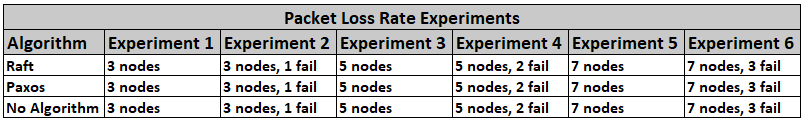
\includegraphics[width=1\textwidth]{LatexSkeleton/images/packet_los_tbl.PNG}
  \caption{Packet Loss Rate Experiments}
\end{table}

\begin{table}[H]
  \centering
  \label{tbl:Latency Experiments}
  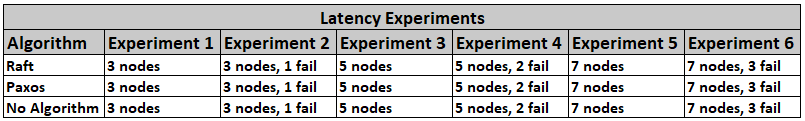
\includegraphics[width=1\textwidth]{LatexSkeleton/images/latency_tbl.PNG}
  \caption{Latency Experiments}
\end{table}
\noindent Building on the work of \cite{Kuipers}, we will implement a limit of 1000 packets to be sent from transmitter nodes to the receiver node during both experiments, with additional decreased number of packets set to simulate nodes’ failures.
\subsection{IoT networks}
Test use cases are planned to be implemented during the first and second control experiment where three networks are created: A, B and C. 

\begin{figure}[H]
\centering
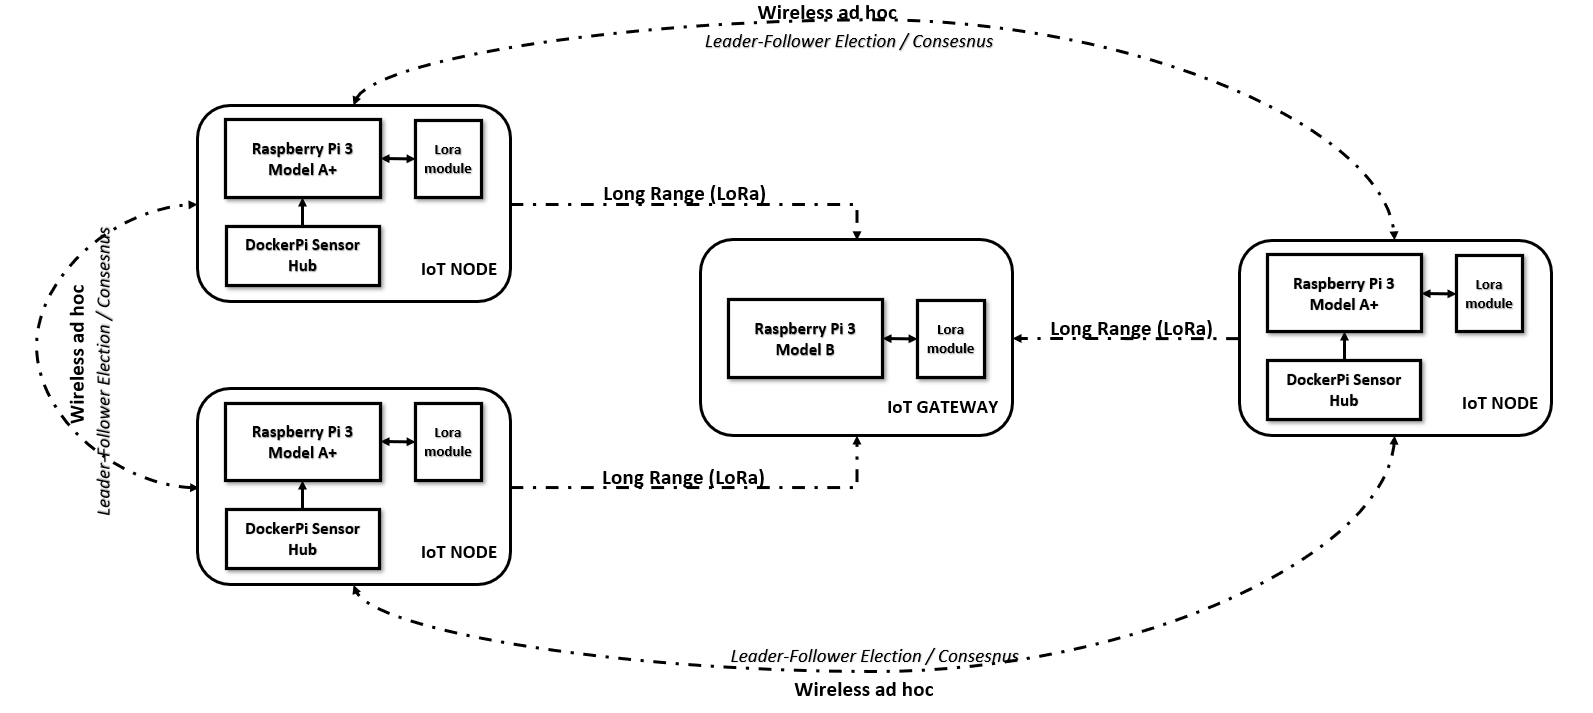
\includegraphics[width=1\textwidth]{LatexSkeleton/images/3_nodes_network.PNG}
\caption{Network A - 3 nodes}
\end{figure}

\begin{figure}[H]
\centering
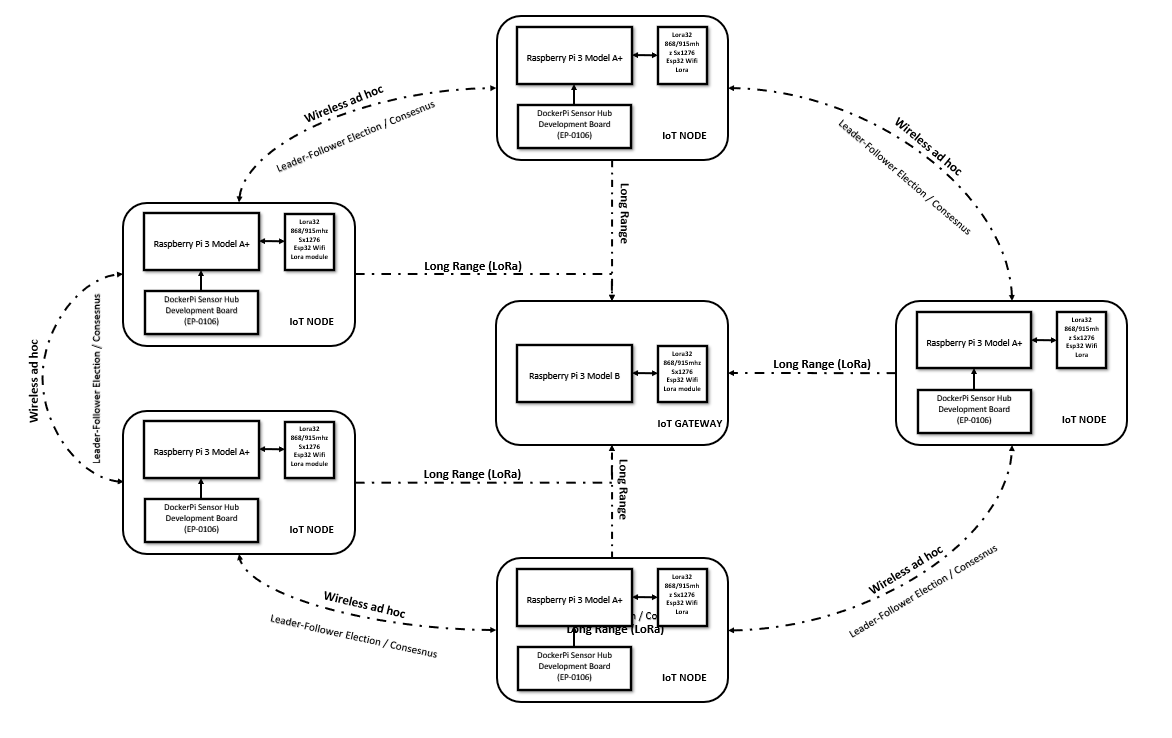
\includegraphics[width=1\textwidth]{LatexSkeleton/images/5_nodes_network.PNG}
\caption{Network B - 5 nodes}
\end{figure}

\begin{figure}[H]
\centering
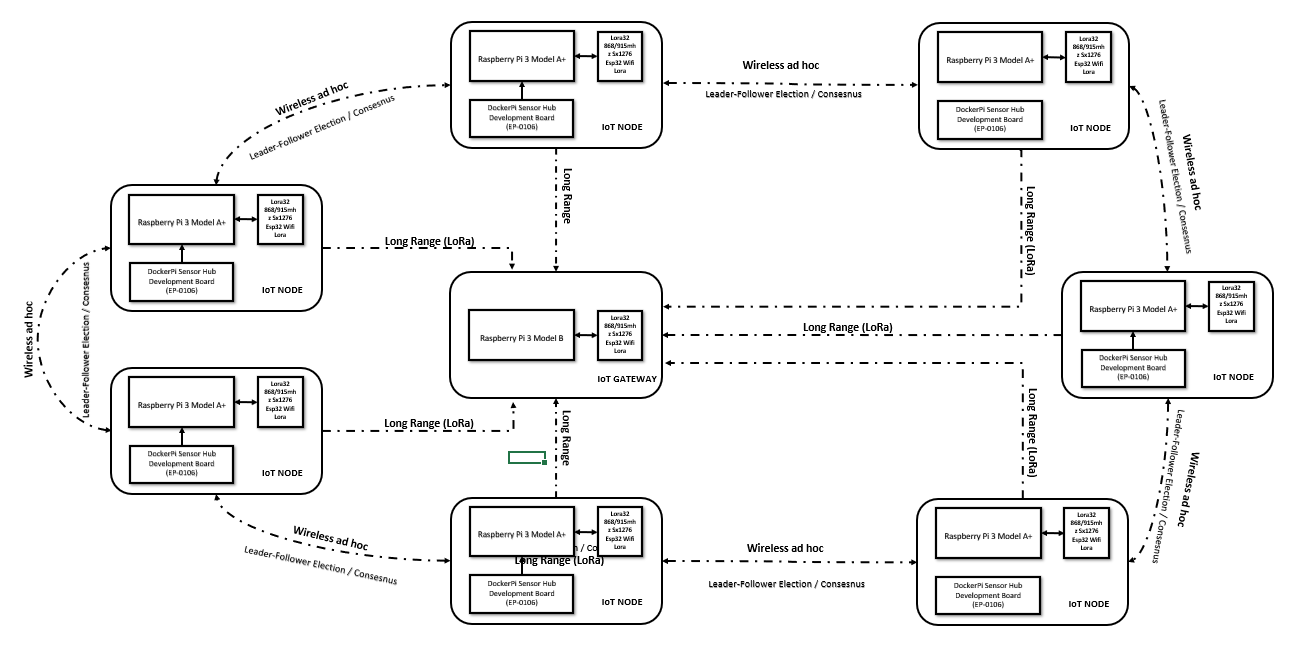
\includegraphics[width=1\textwidth]{LatexSkeleton/images/7_nodes_network.PNG}
\caption{Network C - 7 nodes}
\end{figure}


\noindent Network A will consist of three IoT nodes, Network B of five IoT nodes, and Network C of seven IoT nodes. An odd number of nodes is chosen specifically due to the Paxos and Raft requirement of a minimum number of nodes to achieve consensus \texttt{(N/2 + 1)}.

\subsection{Hardware components}
LoRa is a low-power wide-area network protocol that uses the physical layer of the seven-layer OSI model. The physical layer defines the means of transmitting bits over a physical data link connecting network nodes. LoRa uses unlicensed radio frequencies, including 433 MHz and 868 MHz in the European Union \shortcites{sub-GHz}\citep{sub-GHz}. LoRa enables long-range transmissions with low power consumption, making it a good option for connecting devices in far-reaching environments \citep{CHAUDHARI202015}. As this experiment requires significant amount of hardware components, below section lists each group with detailed specifications.
\subsubsection{IoT nodes}
\myparagraph{Raspberry Pi}
Third-generation Raspberry Pi 3 Model A+ single-board computer (SBC) will serve as an IoT node. It features a Broadcom BCM2837B0, Cortex-A53 (ARMv8) 64-bit SoC @1.4GHz quad-core processor System on a Chip(SoC), 512MB LPDDR2 SDRAM, 2.4GHz and 5GHz IEEE 802.11.b/g/n/ac wireless LAN and Bluetooth 4.2/BLE, Extended 40-pin GPIO header, Single USB 2.0 ports and Micro SD port.
\begin{figure}[H]
\centering
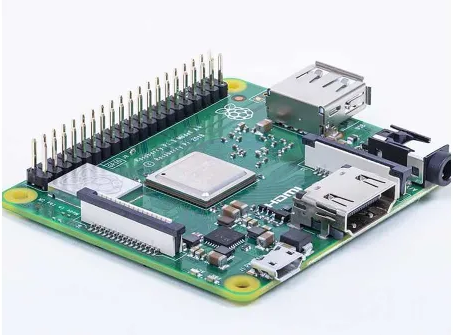
\includegraphics[width=0.5\textwidth]{LatexSkeleton/images/rpi_3a.PNG}
\caption{Raspberry Pi - Model 3A+}
\end{figure}
\myparagraph{Sensor}
Sensor attached to each IoT node is DockerPi Sensor Hub Development Board (EP-0106). It integrates various environmental sensors: temperature sensors, humidity sensors, air pressure sensors, lighting, and thermal imaging sensors. Both, RPP and DockerPi sensor, will be connected using MB102 Breadboard with 3.3V 5V MB102 Breadboard Power Supply Module. 
\begin{figure}[H]
\centering
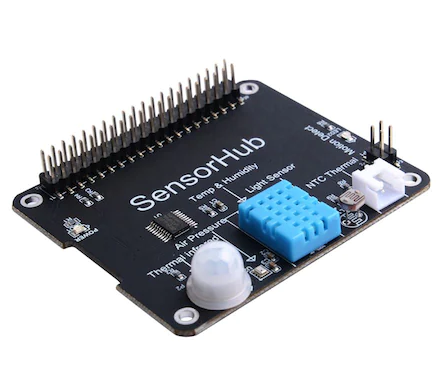
\includegraphics[width=0.5\textwidth]{LatexSkeleton/images/sensor.PNG}
\caption{DockerPi Sensor Hub Development Board}
\end{figure}
\myparagraph{WiFi LoRa ESP32}
Connectivity between edge nodes and gateway will be established with Heltec Lora32 868/915mhz Sx1276 Esp32 WiFi Lora module. WiFi LoRa 32 is an IoT development board produced by Heltec Automation. It is a highly integrated product based on ESP32 microcontroller with 8MB SPI Flash and 529Kb SRAM with SX127x radio chip onboard.  Additionally, it features Wi-Fi, BLE and provides full support for LoRa frequencies.
\begin{figure}[H]
\centering
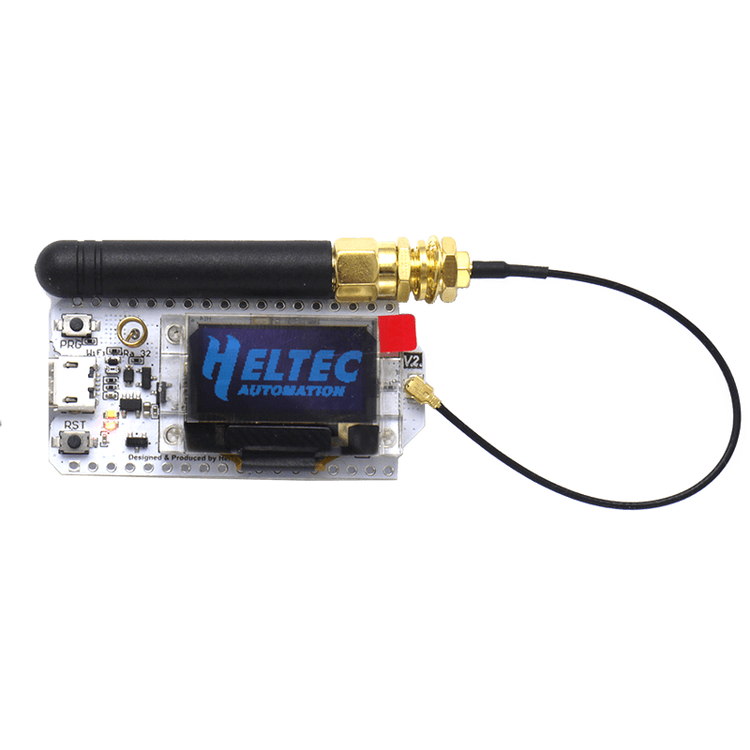
\includegraphics[width=0.5\textwidth]{LatexSkeleton/images/heltec.png}
\caption{ESP32 LoRa Heltec v2 with display}
\end{figure}
\subsection{Python Libraries}
The author of this paper chooses Python programming language to implement Raft and Paxos algorithms.
Python is widely used, and well-documented programming language. Raspberry Pi SBC supports it natively. Additionally, Python libraries provide an implementation of both consensus algorithms. Paxos implementation is based on \cite{composablepaxos} “composable paxos” implementation that provides an algorithmically correct Paxos implementation that can be used in networked applications. Raft implementation used \cite{PySyncObj} “PySyncObj” module that provides the ability to replicate application data between multiple servers.
\subsection{Packet Loss Rate measurement experiment}
\myparagraph{Network A – 3 nodes}
First sub-experiment proposed will measure packet loss rate within IoT network of three nodes. The experiment will be repeated for each of the algorithms, RAFT and Paxos, and additionally for control where no consensus algorithm will be implemented on participating nodes. Packets sent will be recorded on the transmitter and on the receiver node as well and once completed, data will be collected and stored for evaluation and analysis. During the second sub-experiment, fail of one node will be introduced and consequently data will be collected after remaining nodes finished transmitting. 
\myparagraph{Network B – 5 nodes}
Similar steps will be repeated during sub-experiment three, where five IoT nodes will attempt to record and send packets to the receiver node.  The receiver node will record packets that arrived and store them for analysis. These steps shall be repeated for sub-experiment four with the introduction of two faulty nodes stopping transmission independently with different intervals. The results of both experiments will be stored for analysis. Both sub-experiments will be repeated for each of the algorithms and for control without consensus algorithm implemented.
\myparagraph{Network C – 7 nodes}
During sub-experiment six, an IoT network of seven nodes will create data sets by sending packets to the transmitter with RAFT and Paxos algorithms separately implemented and additionally without algorithm. In the course of sub-experiment seven, failures of three nodes will be introduced and data recorded similarly.
Once all data from Packet Loss Rate experiment is collected, it will be analysed in data analysis tool. At this point, the author will be able to draw conclusions on whether the alternative hypothesis H2 and H3 can be accepted or rejected.
\subsection{Latency measurement experiment}
The latency measurement experiment will repeat sub-experiments from the Packet Loss Rate experiment for each IoT network:
\begin{itemize}
  \item Network A – 3 nodes
  \item Network B – 5 nodes
  \item Network C – 7 nodes
\end{itemize}
Additionally, to data collected in the similar way to previous experiment, two timestamps will be added to each packet sent and received. Once having recorded both timestamps, the time it took for data to be transferred between its original source and its destination will be measured, and the author will be able to, either confirm or reject alternative hypothesis H2.
\subsection{Location}
All the above experiments will be carried out in an indoor environment similarly to \cite{Kurji2021}. A utility room of 8 meters long and 7 meters wide, where transmitters will be fixed in the corners. 
\begin{figure}[H]
\centering
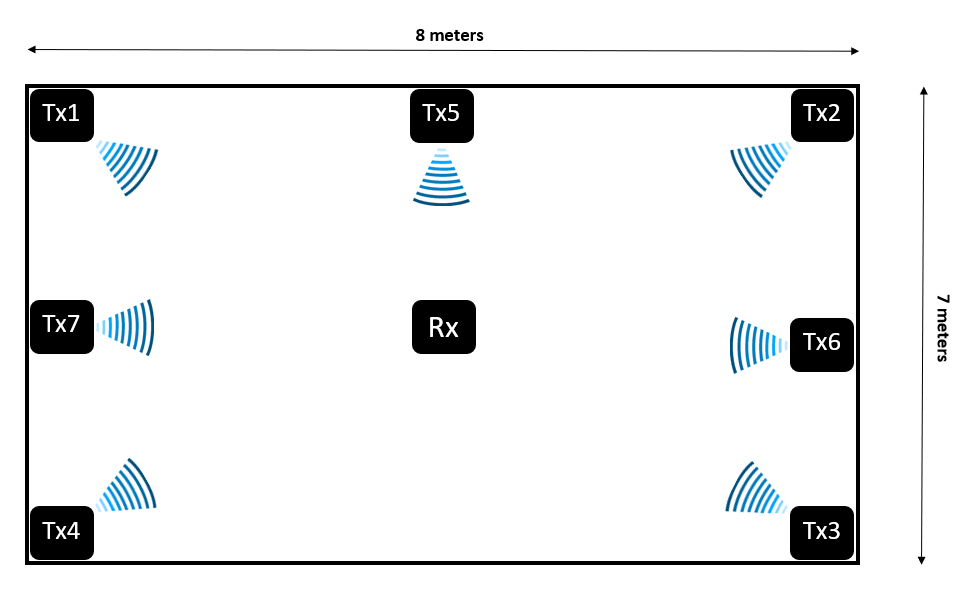
\includegraphics[width=1\textwidth]{LatexSkeleton/images/indoor.PNG}
\caption{Tx and Rx Nodes Setup}
\end{figure}
\noindent Each transmitter will be positioned approximately 1.5 meter above the floor with receiver positioned centrally at around 2 meters height. Below figure  depicts the location of transmitter nodes (Tx) and receiver node (Rx) for Packet Loss Rate and Latency measurements experiments.
\section{Data Design and Data Capture Overview}
During both experiments original (non-existent) quantitative (numerical) data will be collected and analysed to confirm or reject H1, H2, H3 and H4.
\begin{table}[H]
  \centering
  \label{tbl:Packet Loss Rate expected data}
  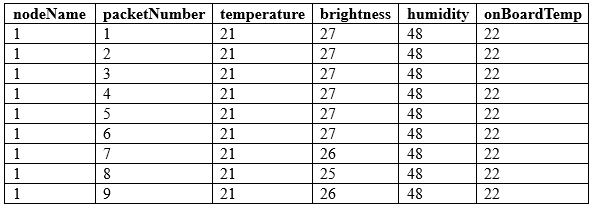
\includegraphics[width=1\textwidth]{LatexSkeleton/images/packet_loss_example_data.PNG}
  \caption{Packet Loss Rate experiment expected data}
\end{table}
\noindent Above data will be recorded on each IoT node (sent packets) and their aggregation is recorded on the receiver node (received packets). The first variable listed in the table, \textbf{nodeName}, represents IoT transmitter node and it will be used to assign \textbf{packetNumber}, variable number two, to each of the transmitters. This will allow identifying packets received and associating them with the correct IoT sender node. Variables three through six will be readings of DockerPi Sensor and their use simulates IoT network deployed in a commercial setting \citep{Kuipers}.
\begin{table}[H]
  \centering
  \label{tbl:Latency experiment expected data}
  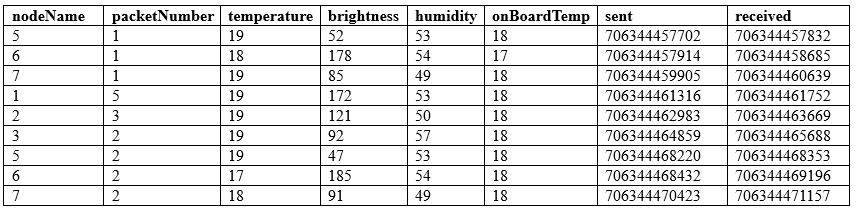
\includegraphics[width=1\textwidth]{LatexSkeleton/images/latency_example_data.PNG}
  \caption{Latency experiment expected data }
\end{table}
 \noindent Variable seven, \textbf{sent}, represents timestamp and will be recorded on the transmitter side for the purpose of the latency measurement experiment. This will be followed by variable eight, \textbf{received}, another timestamp on the receiver’s node side. All data will be saved in CSV files on transmitter and receiver nodes.
 \section{Design and Methodology Summary}
 This section presented an overview of the design and methodology used in the thesis. An overview of the experiment was given, followed by sections that discussed the specifics of the design and methodology. Additionally, data output and capture were discussed, with a detailed evaluation. The next chapter will provide detailed implementation of the experiment.  
% Results, evaluation and discussion chapter
% ============================================================= %
\chapter{Implementation}
\section{Introduction}
This section will build on the previous one by delving deeper into the implementation specifics of experiments and the code required to perform them. The following subsections will be divided based on each component required to execute the test cases.
\section{Required External Libraries}
The below table represents MicroPython and Python 3 external libraries and tools required to conduct experiments for the purpose of this thesis.
\begin{table}[H]
  \centering
  \label{tbl:External Libraries}
  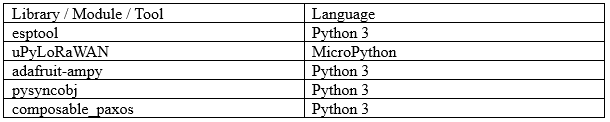
\includegraphics[width=1\textwidth]{LatexSkeleton/images/addit_libraries.PNG}
  \caption{External Libraries }
\end{table}
\section{LoRa Transceiver Board}
\subsection{MicroPython}
WiFi LoRa 32 IoT development board carry the ESP32, a single 2.4 GHz Wi-Fi-and-Bluetooth combo chip, designed for smartwear, mobile and Internet-of-Things (IoT) applications. The ESP32 supports different programming languages, among others is MicroPython, an implementation of Python 3.4 programming language created specifically for microcontrollers. MicroPython, similarly to Python, is easy to use and its  simplified syntax provides more emphasis on natural language. A very important difference between both programming languages is that MicroPython does not come with full standard library but it includes libraries that provide access to low-level hardware like GPIOs. Author decided on using MicroPython for programming of ESP32 on WiFi LoRa 32 IoT development board due to his familiarity with Python and widely available documentation and support.
\subsection{ESP32 Board Set-Up}
Heltec board with ESP32 chip used in these experiments provides dual functionality; it can function as transmitter or receiver. As it is shipped from the producent with Andruino Development Environment preinstalled, it required erasing of the entire flash and deploying MicroPython firmware. This was achieved by connecting the board via USB to the Ubuntu 20.04 OS and using the esptool.py to erase the flash and install new firmware.
\begin{lstlisting}[language=Bash, caption=Firmware installation on ESP32 board,captionpos=b]
#erase flash
sudo python3 esptool.py --chip esp32 --port /dev/ttyUSB1 erase_flash
#install firmware
sudo python3 esptool.py --chip esp32 --port /dev/ttyUSB1 write_flash -z 0x1000 esp32-20220117-v1.18.bin

\end{lstlisting}
Once the board was flashed and MicroPython firmware installed, it required code for the SX127X RF chip and additional helper files to enable LoRa communication. Using ampy tool all required files were transferred onto ESP32 board 
\begin{lstlisting}[language=Bash, caption=File transfer with Ampy tool,captionpos=b]
#transfer files required for enabling LoRa
ampy --port /dev/ttyUSB1 --baud 115200 put config.py
ampy --port /dev/ttyUSB1 --baud 115200 put config_lora.py
ampy --port /dev/ttyUSB1 --baud 115200 put sender.py
ampy --port /dev/ttyUSB1 --baud 115200 put receiver.py
ampy --port /dev/ttyUSB1 --baud 115200 put ssd1306_i2c.py
ampy --port /dev/ttyUSB1 --baud 115200 put ssd1306.py
ampy --port /dev/ttyUSB1 --baud 115200 put sx127x.py
ampy --port /dev/ttyUSB1 --baud 115200 put main.py
ampy --port /dev/ttyUSB1 --baud 115200 put oledsetter.py
\end{lstlisting}
Once files were transferred, board required reset to run main.py with program code.
\subsection{Configuring SX127X RF chip}
Below configuration was chosen for SX127x  based on the work of \cite{8758033} and \cite{Kurji2021}. Spread Factor (SF), bandwidth(BW) and transmission power (Tx) were specifically adopted due to the short distance between the transmitters and the receiver.
\begin{lstlisting}[language=Python, caption=SX127X configuration,captionpos=b]
#configuration required for initialization of SX127x
default_parameters = {
    'frequency': 868E6, 
    'tx_power_level': 2, 
    'signal_bandwidth': 125E3,    
    'spreading_factor': 8, 
    'coding_rate': 5, 
    'preamble_length': 8,
    'implicit_header': False, 
    'sync_word': 0x12, 
    'enable_CRC': False,
    'invert_IQ': False
}
\end{lstlisting}
SX1276x communicates with ESP32 board using Serial Peripheral Interface (SPI) and once SPI is instantiated RF chip is initialized.
\begin{lstlisting}[language=Bash, caption=SPI interface initialization,captionpos=b]
#instantiate SPI interface
board_spi = SPI(baudrate = 115200, 
        polarity = 0, phase = 0, bits = 8, firstbit = SPI.MSB,
        sck = Pin(device_config['sck'], Pin.OUT, Pin.PULL_DOWN),
        mosi = Pin(device_config['mosi'], Pin.OUT, Pin.PULL_UP),
        miso = Pin(device_config['miso'], Pin.IN, Pin.PULL_UP))
#initialize RF chip
lora = SX127x(device_spi, pins=device_config, parameters=lora_parameters)
\end{lstlisting}
\subsection{Communicating with Raspberry Pi}
Universal Asynchronous Receiver/Transmitter. (UART) was chosen as the communication medium between ESP32 and RPi. UART is a hardware communication protocol that uses asynchronous serial communication with configurable speed and requires three wires to enable transmission: a transmit wire, a receive wire, and an electrical ground wire \citep{Embedded}.
\begin{figure}[H]
\centering
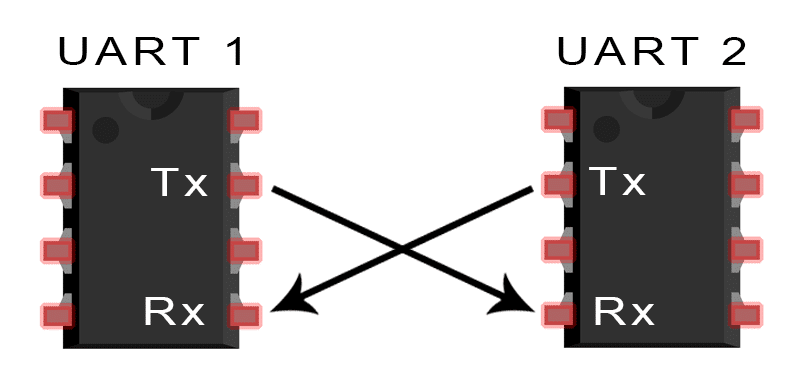
\includegraphics[width=0.5\textwidth]{LatexSkeleton/images/UART-Basic-Connection-Diagram.png}
\caption{UART Basic Connection Diagram}\citep{uart}
\end{figure}
\noindent Both devices, Heltec board and Raspberry Pi, are equipped with a set of GPIOs that allows for straight forward implementation of UART
\begin{lstlisting}[language=Python, caption=UART setup - MicroPython,captionpos=b]
#import UART module from standard library
from machine import UART
#instantiate UART obj
uart = UART(2, 115200)
#initialize UART 
uart.init(115200, bits=8, parity=None, stop=1, tx=17, rx=13)
\end{lstlisting}
\subsection{Transmitting Data}
In order to transmit data, Sender object was instantiated in the main.py on reboot of the ESP32 board. This procedure was repeated on each board designated as transmitter.
\begin{lstlisting}[language=Python, caption=Class Sender - MicroPython,captionpos=b]
class Sender:
    #constructor
    def __init__(self, lora):
        self.lora = lora
    def send(self, msg):
        self.lora.blink_led()
        oled = OledSetter.setOled()
        role = "TRANSMITTER"
        #create payload
        payload = '{p}'.format(p=msg)
        OledSetter.displayOled(oled, role, payload)
        #send payload
        self.lora.println(payload)
\end{lstlisting}
An infinite(while) loop was used for the Sender object to constantly read data from the UART interface and send (\textbf{send()}) it via LoRa and UART interface was used to retrieve messages from Raspberry Pi.
\begin{lstlisting}[language=Python, caption=Instantiation of Sender obj - MicroPython,captionpos=b]
#instantiate Sender obj
sender = Sender(lora)
#infinite loop 
while True:
    #read UART
    msg = uart.readline()
    if msg:
        #send payload
        sender.send(msg)
\end{lstlisting}
Once the ESP32 board was restarted, it automatically accepted any payload sent using the UART interface, smaller than 256 bytes, from Raspberry Pi and immediately sent via LoRa in the ether.
\subsection{Receiving Data}
The receiver object was created in the main.py similarly to the Sender object with the infinite(while) loop in the receive method responsible for reading LoRa packets.
\begin{lstlisting}[language=Python, caption=Class Receiver - MicroPython]
class Receiver:
    #constructor
    def __init__(self, lora):
        self.lora = lora
    
    def receive(lora):
        oled = OledSetter.setOled()
        role = "RECEIVER"
        #infinite loop
        while True:
            if lora.received_packet():
                lora.blink_led()
                #save payload
                payload = lora.read_payload()
                #send payload to UART
                print(payload)
                OledSetter.displayOled(oled, role, payload)
\end{lstlisting}
Heltec LoRa ESP32 board configured as a receiver was constantly accepting packets sent over via LoRa and pushing them using UART interface to Raspberry Pi.
\subsection{Modification to Transmitter and Receiver required for Latency Measurement}
Latency measurement experiment proved to be a challenge due to synchronization issues with internal clocks on both, Raspberry Pi and Heltec LoRa ESP32 boards without access to internet \citep{9035389}. To perform Latency measurement, the author decided on using ESP32 boards WiFi module to synchronize the onboard clock with the Network Time Protocol (NTP) servers to achieve timewise synchronization among the transmitters and receiver boards. Once connected to WiFi on start-up, each node would synchronize its internal time with the local NTP server.
\begin{lstlisting}[language=Python, caption=Synchronization with NTP server for the latency experiment - MicroPython,captionpos=b]
#connect to WiFi
wlan = network.WLAN(network.STA_IF)
wlan.active(True)
wlan.connect('******', '*******')

#sleep until connected to WiFi
while not wlan.isconnected():    
    time.sleep(2)
#synchronize the time of the board
ntptime.settime()
\end{lstlisting}
For the purpose of this thesis, latency was  measured as the difference between timestamps((\textbf{TS}); \texttt{Elapsed Time = TS received {\textminus} TS sent} . To achieve the most accurate results, timestamp was generated on packet sent, in Sender object, and another timestamp was generated on packet received, in Receiver object. Both timestamps were outputted to CSV file on Raspberry Pi to allow for later analysis.   
\begin{lstlisting}[language=Python, caption=Modification of Sender class for the latency experiment - MicroPython,captionpos=b]
#modification to while loop for Sender obj
while True:
    msg = uart.readline()
    if msg:
        #create timestamp in milliseconds
        n = time.time_ns() // 1000000
        sender.send(msg, n)

# modification to while loop for Receiver obj
while True:
        if lora.received_packet():
            #create timestamp in milliseconds
            n = time.time_ns() // 1000000
            lora.blink_led()
            p = lora.read_payload()
            #save payload with the timestamps
            payload = '{m} - {i}'.format(m=p, i=n)
            #send payload to UART
            print(payload)
            OledSetter.displayOled(oled, role, payload)
\end{lstlisting}
\section{Raspberry Pi with DockerPi Hub}
\subsection{Python 3}
Python 3 is a general-purpose interpreted, interactive, object-oriented, and high-level programming language which source code is available under the GNU General Public License. It is a mature language with a large set of comprehensive multipurpose libraries, frameworks and extensions that is actively developed by Python Software Foundation. During the 30 years of existence, Python went through three major revisions and its current version 3.x is not fully backward-compatible with previous iterations. Python’s design was based on concept of modularity, where additional functionality can be added by importing modules instead of building it into the core of the language. The author decided to implement experiments in Python 3 due to its extensibility and the Raspberry Pi operating system being shipped with preinstalled Python 3 onboard. Additionally, as mentioned in the previous subsection, MicroPython is a lighter version of Python 3.4.
\subsection{RPi Operating System}
Raspberry Pi OS (64-bit) v.11, Debian-based operating system, was deployed and running on each Raspberry Pi.
\subsection{RPi Wireless ad hoc network}
Each Raspberry Pi participating in experiments was assigned a static IP address that enabled it to create a part of a   decentralized wireless ad hoc network. To allow connectivity between RPis acting as IoT nodes below changes were made to \texttt{/etc/network/interfaces} file which contains network interface configuration information for Debian Linux.
\begin{lstlisting}[language=Bash, caption=Wireless ad hoc set up,captionpos=b]
#include files from /etc/network/interfaces.d
source-directory /etc/network/interfaces.d
#the loopback network interface
auto lo
iface lo inet loopback
#the primary network interface
iface eth0 inet dhcp
auto wlan0
iface wlan0 inet static
        #assign unique IP address
        address 192.168.1.1
        netmask 255.255.255.0
        wireless-channel 4
        wireless-essid RPIMESH
        wireless-mode ad-hoc
\end{lstlisting}
The table below illustrates the unique IP addresses assigned to each IoT node in ad hoc network: 
\begin{table}[H]
  \centering
  \label{tbl:IP addresses of IoT nodes}
  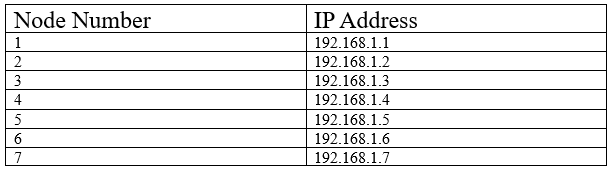
\includegraphics[width=1\textwidth]{LatexSkeleton/images/ip_add.PNG}
  \caption{IP addresses of IoT nodes}
\end{table}
\noindent Once Raspberry Pi was restarted, it automatically joined the wireless ad hoc network and was able to communicate with other nodes in the network.
\subsection{Collecting environmental data with Docker Pi Sensor Hub}
DockerPi Sensor Hub Development Board (EP-0106) was attached to each RPi and together it worked as an IoT node. Sensor Hub was collecting environmental data using various sensors such as: temperature sensors, humidity sensors, air pressure sensors, lighting, and thermal imaging sensors. For the purpose of this thesis author decided to collect four sensor readings (i.e.,  temperature, brightness, humidity and on board temperature) to send them in LoRa packets.
\begin{lstlisting}[language=Python, caption=Sensor data collection - Python3,captionpos=b]
def createData():
    #set registers
    DEVICE_BUS = 1
    DEVICE_ADDR = 0x17
    #set registers
    TEMP_REG = 0x01
    LIGHT_REG_L = 0x02
    LIGHT_REG_H = 0x03
    STATUS_REG = 0x04
    ON_BOARD_TEMP_REG = 0x05
    ON_BOARD_HUMIDITY_REG = 0x06
    ON_BOARD_SENSOR_ERROR = 0x07
    BMP280_TEMP_REG = 0x08
    BMP280_PRESSURE_REG_L = 0x09
    BMP280_PRESSURE_REG_M = 0x0A
    BMP280_PRESSURE_REG_H = 0x0B
    BMP280_STATUS = 0x0C
    HUMAN_DETECT = 0x0D
    
    #initialize System Management Bus
    bus = smbus.SMBus(DEVICE_BUS)

    #container for sensors readings
    aReceiveBuf = []
    aReceiveBuf.append(0x00)
    
    #read registers
    for i in range(TEMP_REG,HUMAN_DETECT + 1):
        aReceiveBuf.append(bus.read_byte_data(DEVICE_ADDR, i))
    
    #return temperature, brightness, humidity, on board temp
    return aReceiveBuf[TEMP_REG], (aReceiveBuf[LIGHT_REG_H] << 8 | aReceiveBuf[LIGHT_REG_L]), aReceiveBuf[ON_BOARD_HUMIDITY_REG], aReceiveBuf[ON_BOARD_TEMP_REG]
\end{lstlisting}
\subsection{Creating LoRa packet and sending it via UART}
Below subsections will illustrate implementation of experiments from chapter three of this thesis. These experiments were divided in three sub experiments based on the algorithm (or lack thereof) used implemented for scheduling purposes. Therefore, control experiments were implemented without any consensus algorithm and were followed by Paxos and Raft consensus algorithms implementations. As the timestamps required for the latency measurement experiment were not added to the packets during program execution on Raspberry Pi, these variables are not presented in the code.  
\myparagraph{Control Experiment}
Listing 4.13 shows how the data is collected from the environmental sensors send to a LoRa ESP32 module and outputted to the CSV file with additional information, i.e., node number and packet number. As per the experiment’s assumptions, the counter variable was initialized and the maximum value was set to 1000 to allow for an exact number of packets to be sent. Every single packet had a unique consecutive number in the range of 1 to 1000 assigned to allow for identification and analysis after the experiments were concluded.
\begin{lstlisting}[language=Python, caption=Control experiment Raspberry Pi code - Python3,captionpos=b ]
def main():
    #set UART serial connection with ESP32
    s = serial.Serial('/dev/ttyS0', 115200)
    #declare node name
    node = 1
    #initialize packet counter
    count = 1
    #declare header for csv file
    header = ['nodeName', 'packetNumber', 'temperature', 'brightness', 'humidity', 'onBoardTemp']  
   
    #create csv file
    with open('sensor-4_data.csv', 'w', encoding='UTF8', newline='') as f:
        #writer object
        writer = csv.writer(f)
        #write the header to the csv file
        writer.writerow(header)

        #loop 
        while True:
            #2 sec interval
            time.sleep(2)        
            #read sensor hub data
            temp, light, humidity, onBoardTemp = createData()
            #create data 
            data = [node, count, temp, light, humidity, onBoardTemp]
            #send packet over UART to LoRa board
            s.write(b'%d,%d,%d,%d,%d,%d' % (node, count, temp, light, humidity, onBoardTemp))
            #save packet to the csv file
	writer.writerow(data)			
            #increment packet counter
            count += 1
\end{lstlisting}
During the control experiments each IoT node, consisting of RPi, sensor hub and LoRa ESP32 board, was collecting and sending data with two seconds intervals and no other mechanism was implemented to prevent packet’s collisions \shortcites{s21041193}\citep{s21041193} or to improve scheduling \shortcites{scheduling}\citep{scheduling}. 
\myparagraph{Paxos Experiment}
Listing 4.14 represents configuration file required to specify nodes of the Paxos group with the IP addresses and ports. This implementation of Paxos require separate files for preserving state of the Paxos group as well.
\begin{lstlisting}[language=Python, caption=Paxos configuration file - Python3,captionpos=b ]
# IP, Port Number
peers = dict(1=(‘192.168.1.1’,12345),2=(‘192.168.1.2’,12345),3=( 192.168.1.3’,12345))

#state files for crash recovery
state_files = dict(1='/tmp/1.json', 2='/tmp/2.json', 3='/tmp/3.json')
\end{lstlisting}
Scheduler in the form of counter was implemented based on consensus and value of the counter was propagated between the nodes participating in the experiment. Once value of the counter was equal to the node number, the packet was sent.
\begin{lstlisting}[language=Python, caption=Paxos experiment Raspberry Pi code - Python3,captionpos=b ]
def main():
    #declare node name
    node = 1
    filename = 'sensor-1_data_raft.csv'
    #initialize Server obj
    serv = Server(node)
    #set serial connection with ESP32
    s = serial.Serial('/dev/ttyS0', 115200)
    #initialize packet counter
    count = 1
    #node counter
    counter = 1
    #declare header for csv file
    header = ['nodeName', 'packetNumber', 'temperature', 'brightness', 'humidity', 'onBoardTemp']  
   
    #create csv file
    with open(filename, 'w', encoding='UTF8', newline='') as f:
        #writer object
        writer = csv.writer(f)
        #write the header to the csv file
        writer.writerow(header)
        #loop 
        while count <= 1000:
            #2 sec interval
            time.sleep(2)
            #check if this node is master node			 
            if serv.get_master() == node:
                if counter <= 3:
                    #increment counter				
                    counter+=1
	        #initialize Client object and propose new value
	        ClientProtocol(node, counter)
                else:
                    #restart counter
                    counter = 1
	        #initialize Client object and propose new value
	        ClientProtocol(node, counter)
	#if the value of the counter matches node number, sent packet		
            if counter == node:
                #read sensor hub data
                temp, light, humidity, onBoardTemp = o.createData()
                #write data to csv file
                data = [node, count, temp, light, humidity, onBoardTemp]
                writer.writerow(data)
                #send packet over lora
                s.write(b'%d,%d,%d,%d,%d,%d' % (node, count, temp, light, humidity, onBoardTemp)) 
            #increment packet count
            count+=1
\end{lstlisting}
\myparagraph{Raft Experiment}
In a similar manner to Paxos algorithm, Raft was implemented with synchronized counter that allowed for scheduling of the packets sent to only one node at the time minimizing collisions of the packets. Two seconds interval was unchanged as per assumption of the control experiment.
\begin{lstlisting}[language=Python, caption=Raft experiment Raspberry Pi code - Python3,captionpos=b ]
def main():
    #this node IP
    my_ip = "192.168.1.1"
    #initialize RaftObj obj
    o = RaftObj('192.168.1.1:12345', ['192.168.1.2:12345', '192.168.1.3:12345'])
    old_value = -1
    filename = 'sensor-1_data_raft.csv'
    #set serial connection with ESP32
    s = serial.Serial('/dev/ttyS0', 115200)
    #declare node name
    node = 1
    #initialize packet counter
    count = 1
    #temp, light, humidity, onBoardTemp = createData()
    #print(node, count, temp, light, humidity, pressure)
    #declare header for csv file
    header = ['nodeName', 'packetNumber', 'temperature', 'brightness', 'humidity', 'onBoardTemp']  
   
    #create csv file
    with open(filename, 'w', encoding='UTF8', newline='') as f:
        #writer object
        writer = csv.writer(f)
        #write the header to the csv file
        writer.writerow(header)
        #loop 
        while count <= 1000:
            #2 sec interval
            time.sleep(2)
            #check if counter is initialized        
            if o.getCounter() != old_value:
                old_value = o.getCounter()
            #check if this node is leader node
            if str(o._getLeader()).split(":", 1)[0] == my_ip:
                if o.getCounter() <= 3: 
                    #increment counter
                    o.addValue(1)
                else:
                    #restart counter
                    o.setCounter(1)
            if o.getCounter() == node:
                #read sensor hub data
                temp, light, humidity, onBoardTemp = o.createData()
                #write data to csv file
                data = [node, count, temp, light, humidity, onBoardTemp]
                writer.writerow(data)
                #send packet over lora
                s.write(b'%d,%d,%d,%d,%d,%d' % (node, count, temp, light, humidity, onBoardTemp)) 
            #increment packet count
            count+=1
\end{lstlisting}
All packets sent during each experiment were outputted to the csv file after forwarding them via UART to the LoRA ESP32 board. The addition of synchronized counter in Paxos and Raft experiments, for the purpose of this thesis functioning as a scheduler, allowed to introduce an order in which packets were sent over LoRa.\smallskip \newline 
Additionally, as per experiments’ requirements, failures of the nodes were carried through changing the packet counter range for nodes 1, 2 and 3 to 300, 500 and 700 correspondingly (dependant on the use case). 
\section{Raspberry Pi Receiver node}
Raspberry Pi acted as the gate node for the purpose of this thesis and, in the similar manner to transmitter nodes, was connected to receiver LoRA ESP32 board via UART. Python script was used to constantly receive any data on the serial port and to output it to csv file. Due to the format of the incoming data some additional string manipulation was required before writing fields to the file. The csv file contained received packets from each node. 
\begin{lstlisting}[language=Python, caption={Receiver Raspberry Pi code - Python3},captionpos=b ]
#set serial connection with ESP32
s=serial.Serial('/dev/ttyS0',115200)
#exclude pattern
pattern = "free"
#declare header for csv file
header = ['nodeName', 'packetNumber', 'temperature', 'brightness', 'humidity', 'onBoardTemp']
#create csv file
with open('/home/bart/msc_python/data.csv', 'w', encoding='UTF8') as f:
    #writer object
    writer = csv.writer(f)
    #write the header to the csv file
    writer.writerow(header)
    #loop
    while True:
        #read input from UART
        data = s.readline()
        #do not process if pattern exists
        if data and not re.search(pattern, data.decode()):
            #decode from bytestream
            d = data.decode()
	#cleanup
            final_data = d.replace('"','').replace("b","").replace("'", "").replace("\r","").replace("\n","").replace("-",",").replace(" ","")
            #write data to the file
	writer.writerow(final_data.split(","))
\end{lstlisting}
\section{Conclusion}
In this chapter author covered in depth the implementations of the experiments with detailed code examples and discussed the setup of each of the components required to perform them. The next section will discuss the results obtained from the experiments.
% Chapter 5 chapter
% ============================================================= %
\chapter{Results, Evaluation and Discussion}
\section{Introduction}
This section discusses the results obtained from running the experiments described in detail in Chapters Three and Four. Results from the Packet Loss Rate  and Latency implementations will be presented and compared. This Chapter will also evaluate the results, with some discussion taking place.
\section{Research Question}
Can implementation of Raft consensus algorithm in IoT network decrease packet loss rate and improve latency on the network in the presence of malfunctioning edge nodes when compared to Paxos consensus algorithm?
\section{Results}
\subsection{Packet Loss Rate measurement experiment}
\myparagraph{Test Statistics}
T-test with paired-samples was used to statistically compare performance of consensus algorithms during experiments with different conditions. Author attempted to calculate \texttt{p-value} to either confirm or reject null hypothesis. \texttt{P-value} indicates if the difference between two paired samples is statistically significant. As level of statistical significance is denoted by the value between 0 and 1, higher \texttt{p-value} indicate that null hypothesis should be accepted and rejected in case of smaller \texttt{p-value}:
\begin{itemize}
  \item \texttt{p-value} higher than 0.05 is not statistically significant (\texttt{p-value $>$ 0.05})   
  \item \texttt{p-value} less than 0.05 is statistically significant (\texttt{p-value $\leq$ 0.05})
\end{itemize}
\begin{table}[H]
  \centering
  \label{tbl:p-values}
  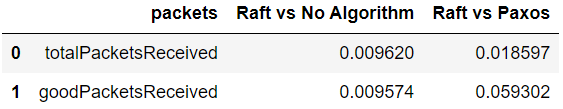
\includegraphics[width=0.6\textwidth]{LatexSkeleton/images/p-values.PNG}
  \caption{\texttt{p-values}}
\end{table}
In the above table the p-value clearly demonstrates that the null hypothesis can be rejected for IoT network with no consensus algorithm implemented. P-value for Paxos implementation signifies that null hypothesis should be accepted. These results of t-test are expected, as both consensus algorithms introduce order to LoRa transitions hence decreasing Packet Loss Rate. 
\myparagraph{Experiments’ evaluation}
Attempted indoor control experiments, with no consensus algorithm implemented, delivered results where packet loss rate was notably high when compared to author’s expectations.
\begin{table}[H]
  \centering
  \label{tbl:Indoor control experiments results}
  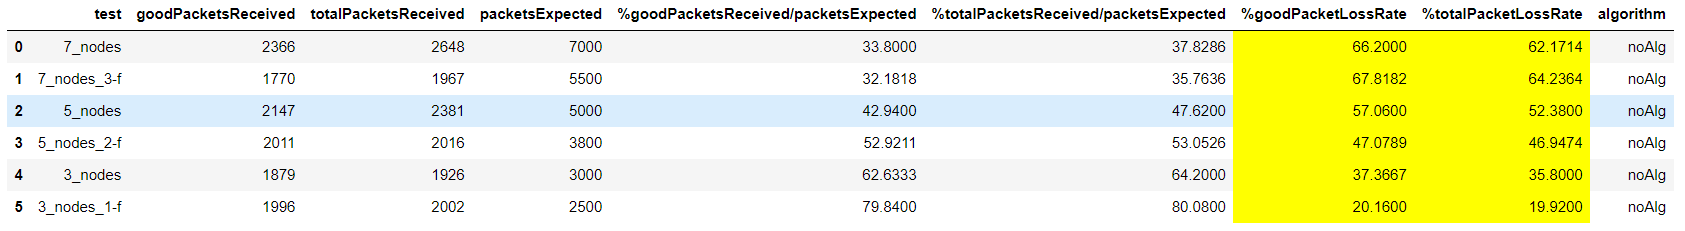
\includegraphics[width=1\textwidth]{LatexSkeleton/images/indoor_only.PNG}
  \caption{Indoor control experiments results}
\end{table}
\noindent After further research, author realized that, as per \cite{BuildingEnvironments} “the packet loss rate in the outdoor under line-of-sight environment was much smaller than that in the indoor environment”. Following on these findings, all experiments were redesigned and relocated outdoors. Locations of the nodes were adjusted due to topography of the outdoor space.  
\begin{figure}[H]
    \centering
    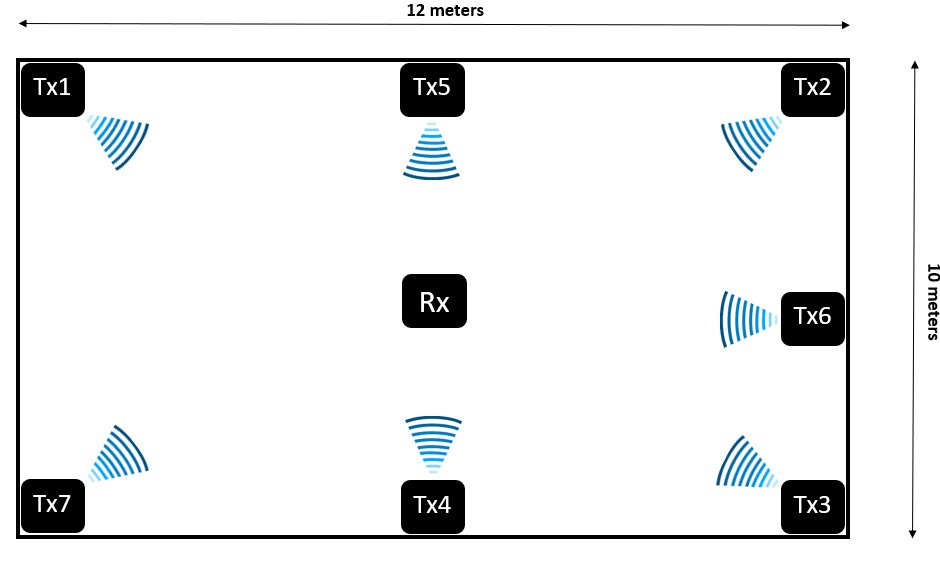
\includegraphics[width=0.6\textwidth]{LatexSkeleton/images/outdoor.PNG}
    \caption{Outdoor Tx and Rx Nodes Setup}
\end{figure}
\noindent Additionally due to the collisions of the LoRa packets \citep{Collisions}, the data received required additional steps to remove corrupted and incorrectly formatted data from the data set. Example in the table below shows corrupted and incomplete data in dataset created on the receiver side.
\begin{table}[H]
  \centering
  \label{tbl:Errors in data due to collisions}
  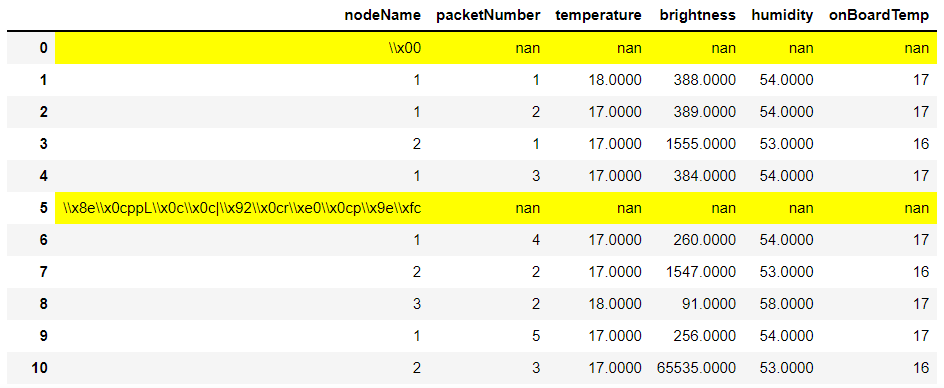
\includegraphics[width=0.6\textwidth]{LatexSkeleton/images/errors_in_data.PNG}
  \caption{Errors in data due to collisions}
\end{table}
\noindent Once data cleansing process was completed, data set contained only numerical values assigned to six columns of which column \textbf{nodeName} and column \textbf{packetNumber} were analysed for the purpose of the Packet Loss Rate experiment.
\begin{table}[H]
  \centering
  \label{tbl:nodeName and packetNumber columns}
  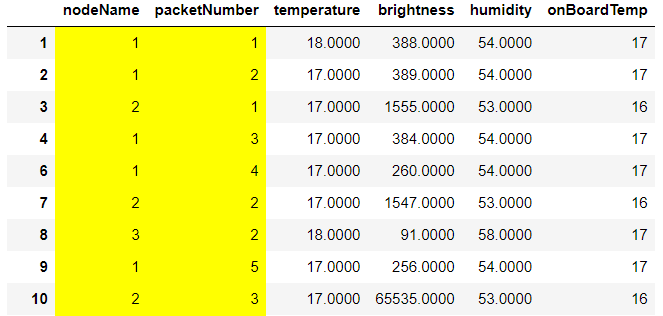
\includegraphics[width=0.6\textwidth]{LatexSkeleton/images/2_columns_only.PNG}
  \caption{\textbf{nodeName} and \textbf{packetNumber}}
\end{table}
\noindent Below subsections will present the measurement of the frequencies of each node in the dataset representing packets received. As each node transmitted exactly 1000 packets, the packet loss rate was measured by multiplying number of packets sent by the number of nodes participating in the experiment. Numbers are represented in three columns per each experiment: 
\begin{itemize}
  \item \textbf{goodPacketsReceived} representing data after cleaning of the dataset
  \item \textbf{totalPacketsReceived} representing all rows in the dataset
  \item  \textbf{packetsExpected} representing number of expected packets
\end{itemize}
To simulate failing nodes during experiments, below configuration was applied. Once the transmitter node reached pre-set limit of packets to be sent, it would automatically switch off:
\begin{table}[H]
  \centering
  \label{tbl:Packet limit at which nodes would turn off to simulate failure}
  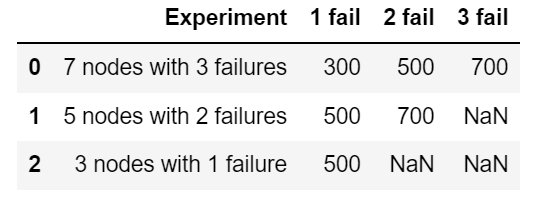
\includegraphics[width=0.6\textwidth]{LatexSkeleton/images/failures_per_exp.png}
  \caption{Packet limit at which nodes would turn off to simulate failure}
\end{table}
\noindent By removing randomness from the experiments requiring node failures, author attempted to introduce predictable number of packets expected.  
\myparagraph{Network A – 3 Nodes}
During the first sub-experiment author measured the packet loss rate within IoT network of three nodes. The experiment was repeated for each of the consensus algorithms, RAFT and Paxos, and additionally for control where no consensus algorithm was implemented on participating nodes. Each of the transmitter nodes recorded 1000 environmental readings and attempted to dispatch them  via LoRa medium. All packets sent were recorded on the transmitter and on the receiver node as well, in csv format, to allow for further evaluation and analysis in Jupyter Notebook.\smallskip \newline
In the second sub-experiment, the failure of one node was introduced to measure the impact on LoRa traffic and packet loss rate. Similarly, all packets sent and received were recorded and evaluated in Jupyter Notebook during the experiment evaluation phase.\smallskip \newline
\textbf{3 Nodes, no node failure}\smallskip \newline
Figure \ref{fig:3 Nodes, no node failure} shows the number of packets received during each experiment, i.e., Raft implementation, Paxos implementation and no algorithm. In this experiment author expected 3000 thousand packets to be recorded in dataset on the receiver node. It can be seen from the figure that both implementations of consensus algorithm, Raft and Paxos, significantly decrease packet loss rate. 
\begin{figure}[H]
    \centering
    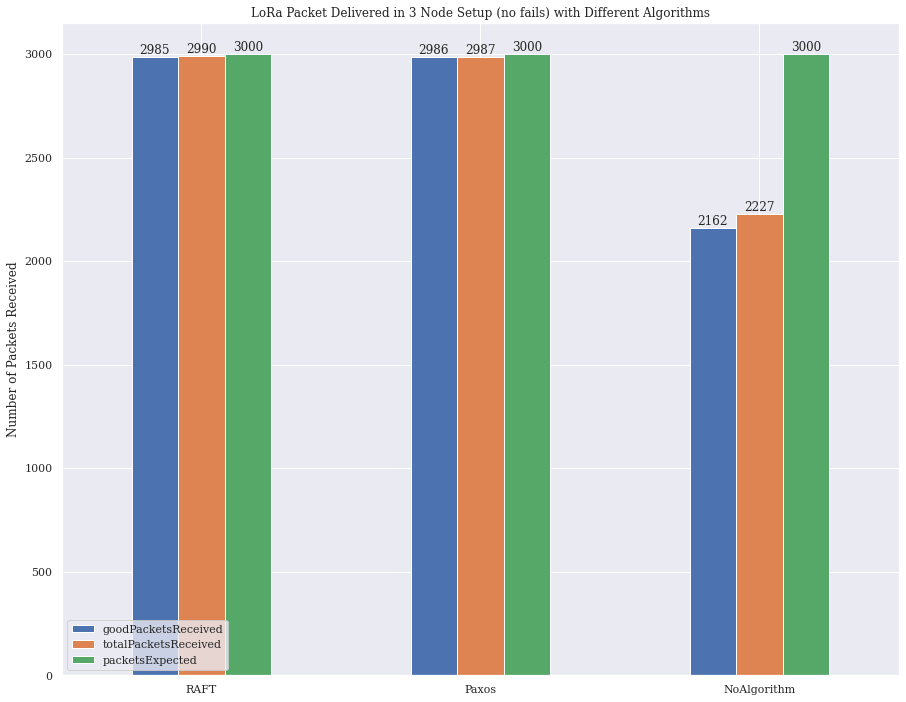
\includegraphics[width=0.6\textwidth]{LatexSkeleton/images/3_nodes.png}
    \caption{3 Nodes, no node failure}\label{fig:3 Nodes, no node failure}
\end{figure}
\noindent Both, IoT network with Raft and Paxos, achieved over 99\% of the packets delivered successfully and their performance was better than the IoT network without any consensus implementation.
\begin{table}[H]
  \centering
  \label{tbl:3 Nodes, no node failure}
  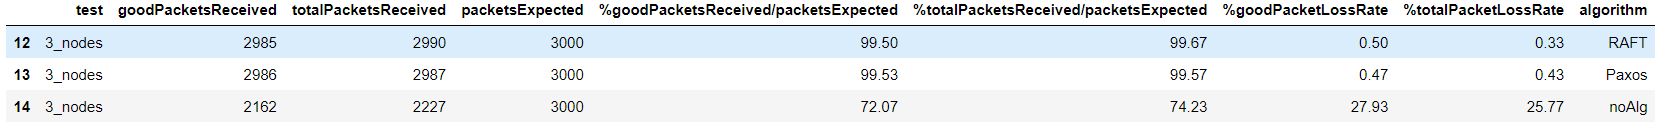
\includegraphics[width=1\textwidth]{LatexSkeleton/images/3_nodes_percentage.PNG}
  \caption{3 Nodes, no node failure}
\end{table}
\noindent\textbf{3 Nodes, 1 node failure}\smallskip \newline
During experiment with three nodes and one failure simulated at 500 packets, we can see from Figure \ref{fig:3 Nodes, 1 node failure} that it very closely follows Figure 5.2 in respect to Raft algorithm. Paxos implementation result, although not as efficient as Raft implementation, is showing a significant advantage in decreasing packet loss rate when compared to no consensus implementation as well.
\begin{figure}[H]
    \centering
    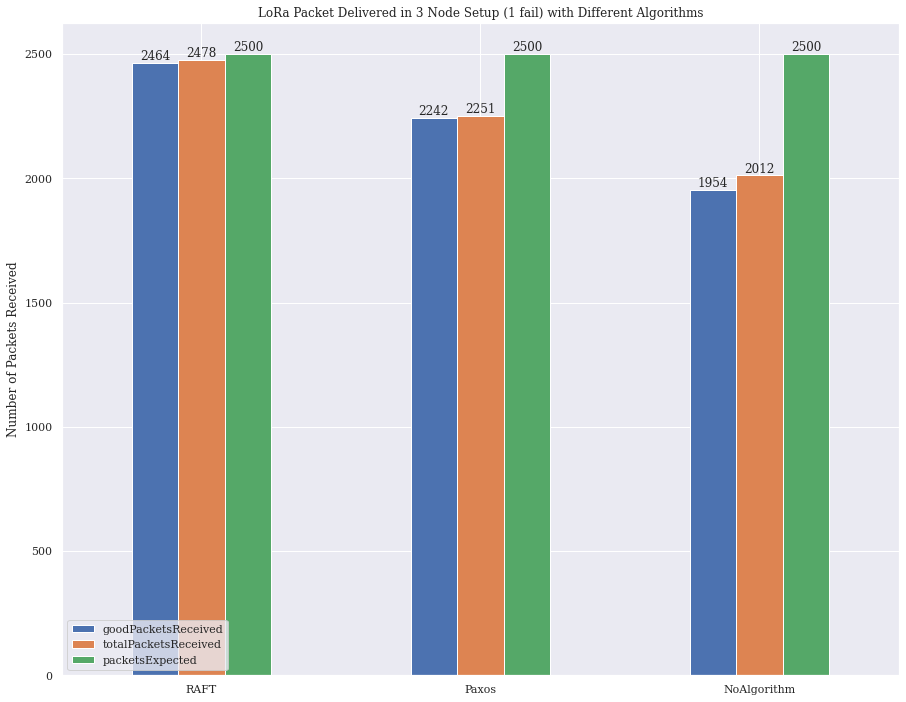
\includegraphics[width=0.6\textwidth]{LatexSkeleton/images/3_nodes_1.png}
    \caption{3 Nodes, 1 node failure}\label{fig:3 Nodes, 1 node failure}
\end{figure}
\noindent As can be seen from Table \ref{tbl:3 Nodes, 1 node failure}, Raft consensus algorithm implementation decreases packet loss rate when compared to no implementation in control experiment.
\begin{table}[H]
  \centering
  \caption{3 Nodes, 1 node failure}
  \label{tbl:3 Nodes, 1 node failure}
  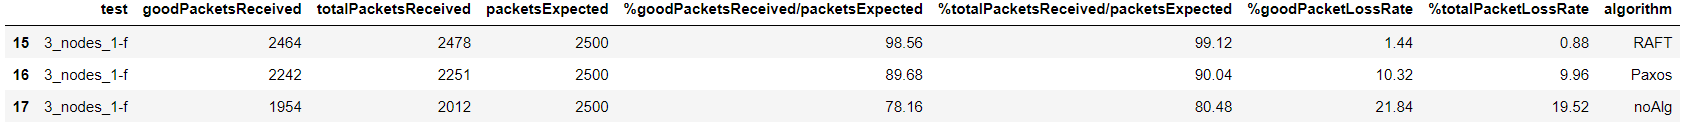
\includegraphics[width=1\textwidth]{LatexSkeleton/images/3_nodes_1-f_percentage.png}
\end{table}
\myparagraph{Network B – 5 Nodes}
Similar steps were repeated during sub-experiment three, where five IoT nodes attempted to record and send packets to the receiver node.  The receiver node recorded packets that arrived and stored them for analysis. These steps were repeated for sub-experiment four with the introduction of two faulty nodes stopping transmission independently with different intervals. Results of both experiments were stored for analysis in a csv file on transmitter and receiver nodes. Both sub-experiments were repeated for each of the algorithms and for control without a consensus algorithm implemented. 
\noindent\textbf{5 Nodes, no node failure}\smallskip \newline
Figure \ref{fig:5 Nodes, no node failure} represents number of packets received in experiments with 5 nodes. Once again, it shows that general trend of Raft algorithm decreasing packet loss rate is upheld. 
\begin{figure}[H]
    \centering
    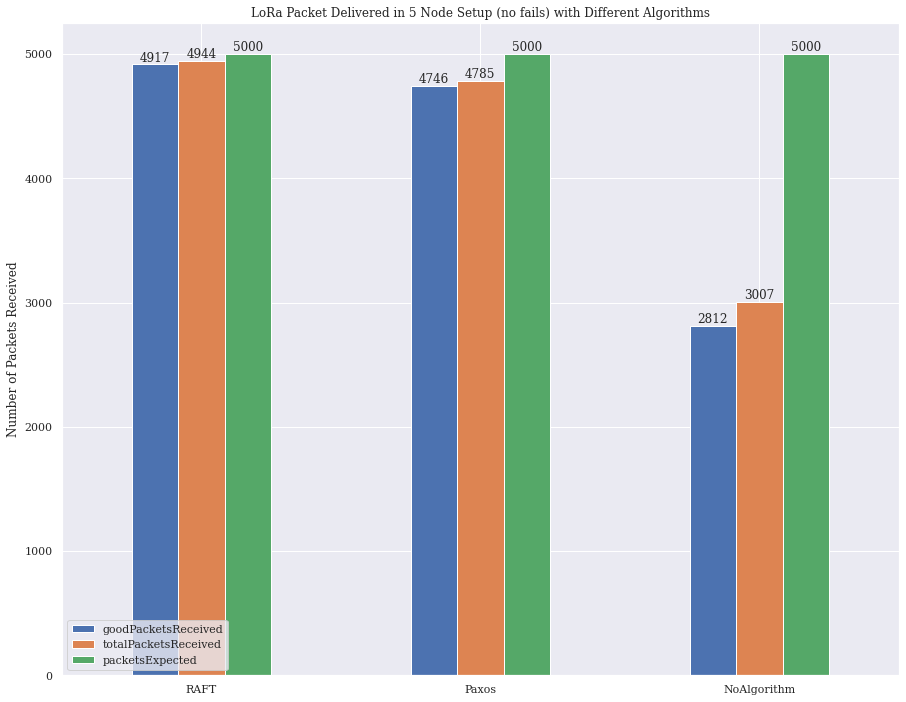
\includegraphics[width=0.6\textwidth]{LatexSkeleton/images/5_nodes.png}
    \caption{5 Nodes, no node failure}\label{fig:5 Nodes, no node failure}
\end{figure}
\noindent During experiments IoT network with Raft implementation achieved over 98\% of packet delivery rate, followed closely by Paxos implementation.
\begin{table}[H]
  \centering
  \label{tbl:5 Nodes, no node failure}
  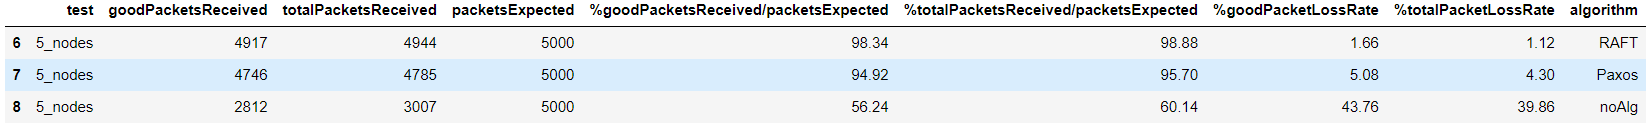
\includegraphics[width=1\textwidth]{LatexSkeleton/images/5_nodes_percentage.PNG}
  \caption{5 Nodes, no node failure}
\end{table}
\noindent\textbf{5 Nodes, 2 node failures}\smallskip \newline
Similarly, when 2 failures were introduced, IoT network with Raft implementation significantly outperforms IoT network without consensus algorithm implementation. Figure \ref{fig:5 Nodes, 2 node failures} shows packets delivered during experiments with both algorithms implemented and control experiment.
\begin{figure}[H]
    \centering
    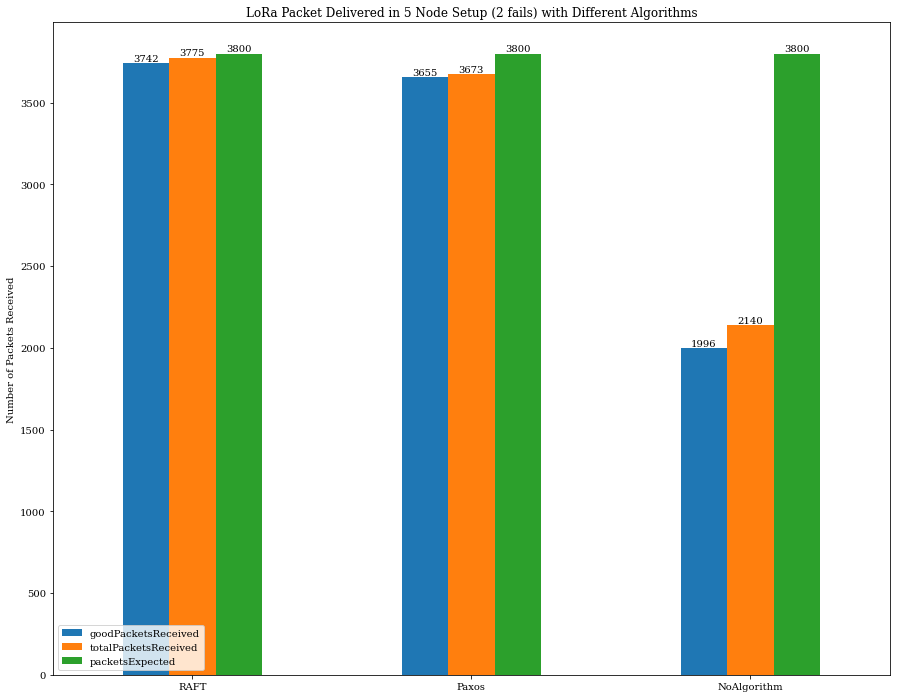
\includegraphics[width=0.6\textwidth]{LatexSkeleton/images/5_nodes_2.png}
    \caption{5 Nodes, 2 node failures}\label{fig:5 Nodes, 2 node failures}
\end{figure}
\noindent During this experiment both consensus algorithms outperformed IoT network without algorithm implementation, as can be seen in Figure \ref{fig:5 Nodes, 2 node failure}.
\begin{table}[H]
  \centering
  \label{tbl:5 Nodes, 2 node failure}
  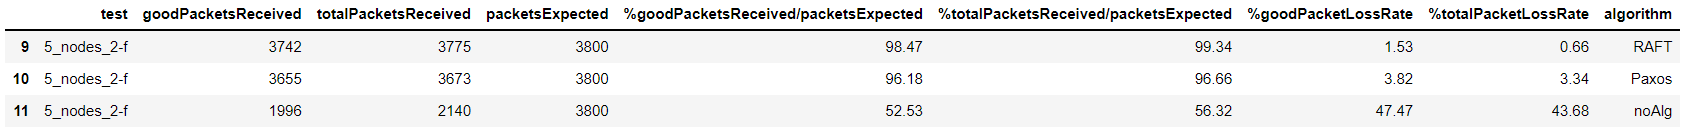
\includegraphics[width=1\textwidth]{LatexSkeleton/images/5_nodes_2-f_percentage.PNG}
  \caption{5 Nodes, 2 node failure}\label{fig:5 Nodes, 2 node failure}
\end{table}
\myparagraph{Network C – 7 nodes}
During sub-experiment six, IoT network of seven nodes created data sets by sending packets to transmitter with Raft and Paxos algorithms separately implemented and additionally without algorithm. During sub-experiment seven, failures of three nodes were introduced and data were recorded in CSV format, in similar manner to the previous experiments.\smallskip \newline
Once all data from the Packet Loss Rate experiment was collected, the author analysed it in Jupyter Notebook tool and at this point, the author was able to draw conclusions on whether the alternative hypotheses H2 and H3 can be accepted or rejected.
\noindent\textbf{7 Nodes, no node failure }\smallskip \newline
Figure \ref{fig:7 Nodes, no node failures} shows results of the experiments with 7 nodes where both IoT networks with implemented algorithms show clear advantage in respect to decreasing packet loss rate in comparison to IoT network from control experiment.  
\begin{figure}[H]
    \centering
    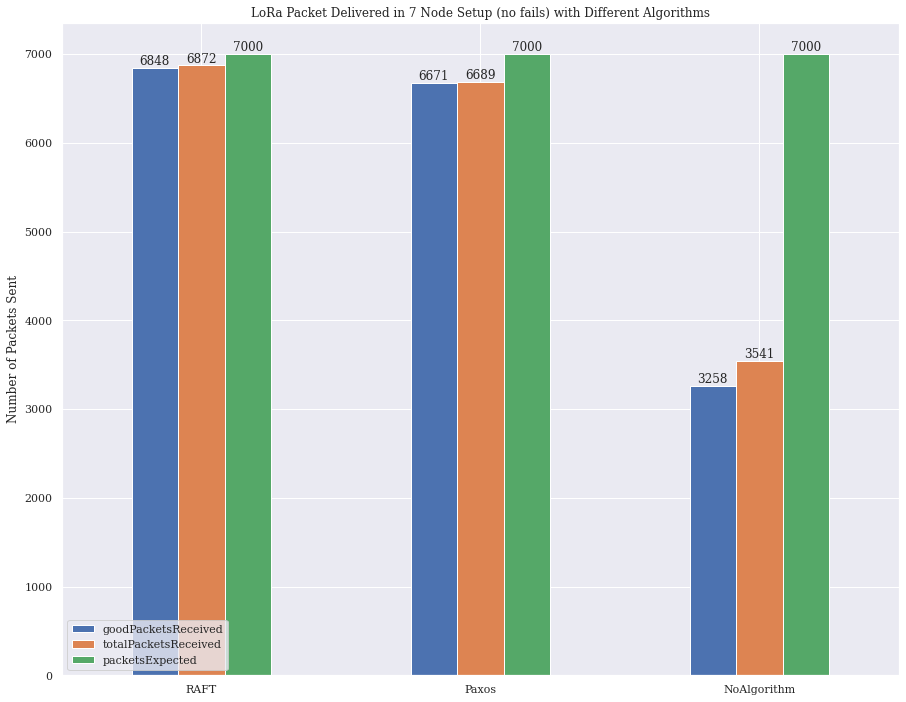
\includegraphics[width=0.6\textwidth]{LatexSkeleton/images/7_nodes.png}
    \caption{7 Nodes, no node failures}\label{fig:7 Nodes, no node failures}
\end{figure}
\noindent Likewise, when the percentage of packets delivered is shown in Table \ref{tbl:7 Nodes, no node failure} it demonstrates the advantage of implementing a consensus algorithm in IoT network. Both algorithms deliver a packet loss rate of less than 5\%.
\begin{table}[H]
  \centering
  \label{tbl:7 Nodes, no node failure}
  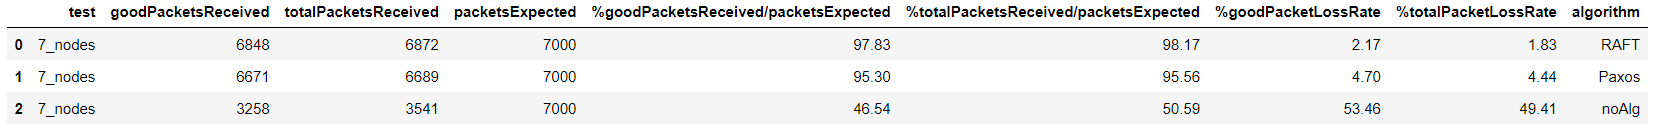
\includegraphics[width=1\textwidth]{LatexSkeleton/images/7_nodes_percentage.PNG}
  \caption{7 Nodes, no node failure}
\end{table}
\noindent\textbf{7 Nodes, 3 node failures}\smallskip \newline
Figure \ref{fig:7 Nodes, 3 node failures} represents the results of the final sub-experiments in Packet Loss Rate measurement experiment.
\begin{figure}[H]
    \centering
    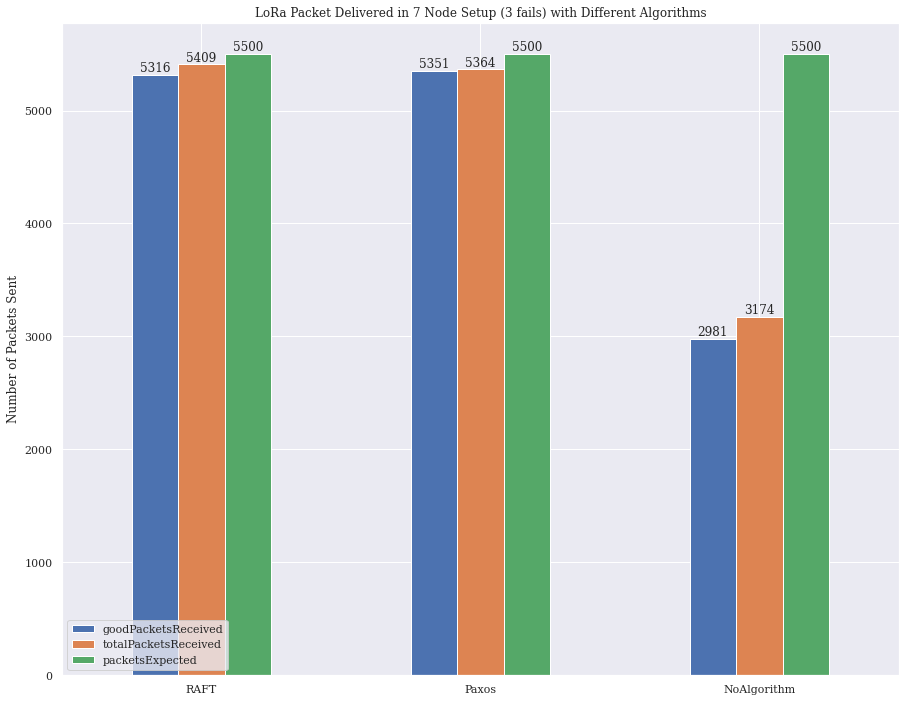
\includegraphics[width=0.6\textwidth]{LatexSkeleton/images/7_nodes_3.png}
    \caption{7 Nodes, 3 node failures}\label{fig:7 Nodes, 3 node failures}
\end{figure}
\noindent Following on similar trend shown in previous experiments, both consensus algorithms  provide significant advantage in respect to delivering decrease in packet loss rate in IoT network.
\begin{table}[H]
  \centering
  \label{tbl:7 Nodes, 3 node failure}
  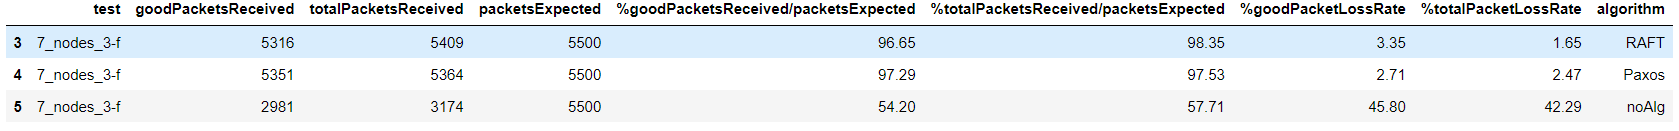
\includegraphics[width=1\textwidth]{LatexSkeleton/images/7_nodes_3-f_percentage.PNG}
  \caption{7 Nodes, 3 node failure}
\end{table}
\subsection{Latency measurement experiment}
Latency measurement experiment repeated all sub-experiments from Packet Loss Rate experiment for each IoT network:
\begin{itemize}
  \item Network A – 3 nodes
  \item Network B – 5 nodes
  \item Network C – 7 nodes
\end{itemize}
\noindent Additionally, to data collected in the similar way to previous experiment, two timestamps were added to each packet send and received. Once having recorded both timestamps, the time it took for data to be transferred between its original source and its destination was calculated. 
\myparagraph{Experiments’ evaluation}
Datasets retrieved from Receiver node required additional cleaning due to number of empty or corrupted rows. 
\begin{table}[H]
  \centering
  \label{tbl:Errors in dataset }
  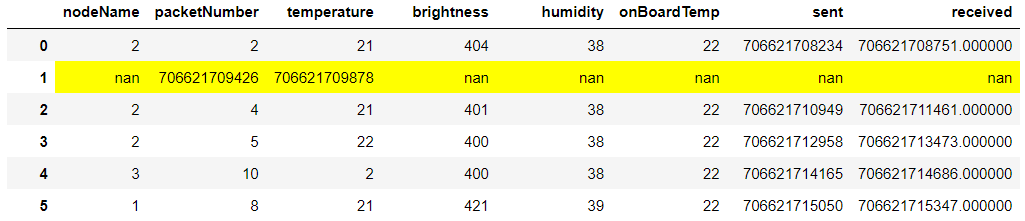
\includegraphics[width=1\textwidth]{LatexSkeleton/images/errors_in_data_latency.PNG}
  \caption{7 Nodes, 3 node failure}
\end{table}
\noindent As latency, or delay is calculated as the difference between received timestamp and sent timestamp, the author decided to discard all columns bar two: \textbf{sent} and \textbf{received}.
\begin{table}[H]
  \centering
  \label{tbl:Timestamps for latency experiment}
  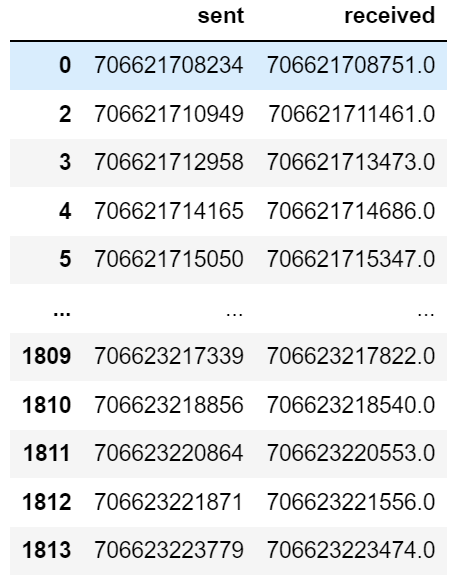
\includegraphics[width=0.2\textwidth]{LatexSkeleton/images/set_received_only.PNG}
  \caption{Timestamps for latency experiment}
\end{table}
\noindent Below figures represent latency measurement taken during repeated experiments where timestamp was concatenated on transmitter node and additional timestamp was added when packet was received on receiver IoT node.
\begin{figure}[H]
\centering
\begin{subfigure}{.5\textwidth}
  \centering
  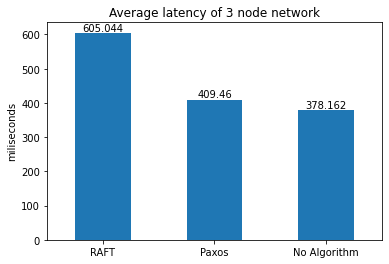
\includegraphics[width=.9\linewidth]{LatexSkeleton/images/latency_3_mean.png}
  \caption{3 Nodes, no node failure latency}
  \label{fig:3 Nodes, 1 node failure latency}
\end{subfigure}%
\begin{subfigure}{.5\textwidth}
  \centering
  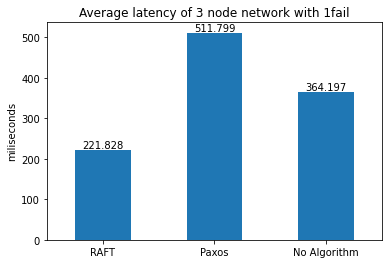
\includegraphics[width=.9\linewidth]{LatexSkeleton/images/latency_3_1_mean.png}
  \caption{3 Nodes, 1 node failure latency}
  \label{fig:3 Nodes, 1 node failure latency}
\end{subfigure}
\caption{Latency in Network A – 3 nodes}
\label{fig:test}
\end{figure}
\begin{figure}[H]
\centering
\begin{subfigure}{.5\textwidth}
  \centering
  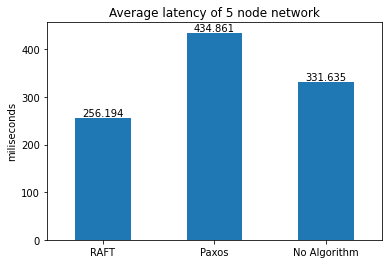
\includegraphics[width=.9\linewidth]{LatexSkeleton/images/latency_5_mean.png}
  \caption{5 Nodes, no node failure latency}
  \label{fig:5 Nodes, no node failure latency}
\end{subfigure}%
\begin{subfigure}{.5\textwidth}
  \centering
  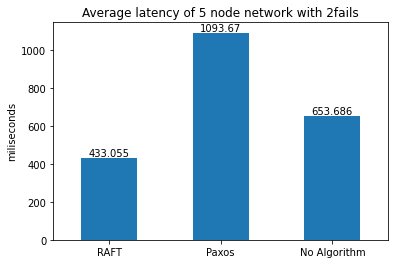
\includegraphics[width=.9\linewidth]{LatexSkeleton/images/latency_5_2_mean.png}
  \caption{5 Nodes, 2 node failure latency}
  \label{fig:5 Nodes, 2 node failure latency}
\end{subfigure}
\caption{Latency in Network B – 5 nodes}
\label{fig:test}
\end{figure}
\begin{figure}[H]
\centering
\begin{subfigure}{.5\textwidth}
  \centering
  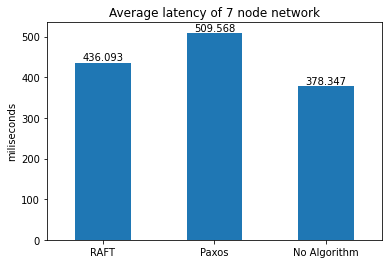
\includegraphics[width=.9\linewidth]{LatexSkeleton/images/latency_7_mean.png}
  \caption{7 Nodes, no node failure latency}
  \label{fig:7 Nodes, no node failure latency}
\end{subfigure}%
\begin{subfigure}{.5\textwidth}
  \centering
  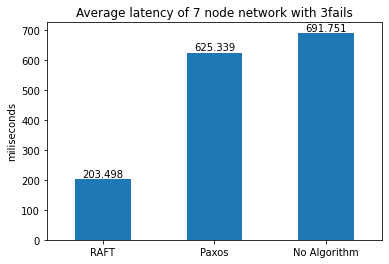
\includegraphics[width=.9\linewidth]{LatexSkeleton/images/latency_7_3_mean.png}
  \caption{7 Nodes, 3 node failure latency}
  \label{fig:7 Nodes, 3 node failure latency}
\end{subfigure}
\caption{Latency in Network C – 7 nodes}
\label{fig:test}
\end{figure}
Additionally, Figure \ref{fig:Average latency of all networks (A, B and C)} shows each latency value plotted on the same diagram with the results comparable to the ones achieved by \cite{8758033} in their work on end-to-end latency of LoRaWAN. 
\begin{figure}[H]
    \centering
    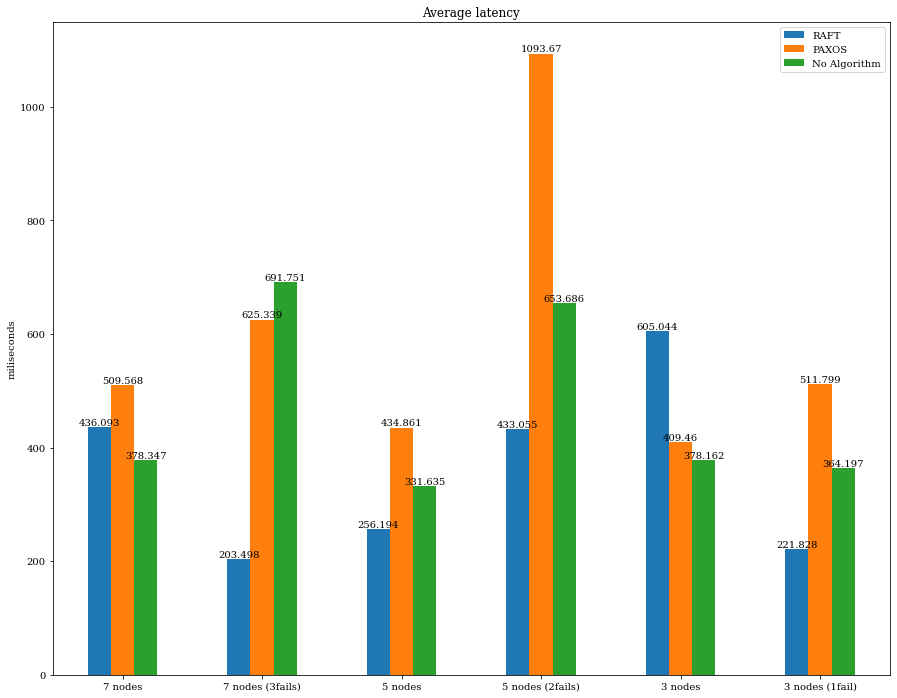
\includegraphics[width=0.6\textwidth]{LatexSkeleton/images/average_latency_all_nodes.png}
    \caption{Average latency of all networks (A, B and C)}\label{fig:Average latency of all networks (A, B and C)}
\end{figure}
\noindent As demonstrated in previous figures, IoT networks with Raft implementation have an advantage (in most cases) in regards to decreasing latency on IoT networks, over IoT networks with either Paxos implementation or no consensus algorithm at all.  
\begin{table}[H]
  \centering
  \label{tbl:Average latency of all networks (A, B and C) }
  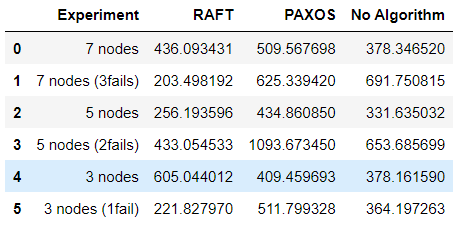
\includegraphics[width=0.4\textwidth]{LatexSkeleton/images/latency_all.PNG}
  \caption{Average latency of all networks (A, B and C)}
\end{table}
\section{Discussion}
\subsection{Results Evaluation}
From the results in Packet Loss Rate experiment section, author can clearly see that there is an advantage in implementing Raft consensus algorithm on IoT networks to decrease possible packet loss rate. Not surprisingly, Paxos consensus algorithm implementation delivers similar results as Raft algorithm. Both networks with consensus algorithms implemented scheduling mechanisms that used synchronized counter to introduce order in the packets’ expedition. Once possibility of packet collisions was minimized by allowing only one node to send packets at given time, this significantly reduces lost packets. Packet loss experiments focused on deliverability of the message and in all test cases, their results proved that scheduling by implementing consensus algorithm has potentially huge benefits. This partially answers the research question related to decreasing packet loss rate by implementing Raft on IoT networks by proving that Raft implementation can potentially deliver huge benefits for LoRa operators.\smallskip \newline 
In terms of decreasing latency in IoT network with the help of Raft consensus algorithm, the author has to admit that, although results clearly point to the advantage of Raft over Paxos and IoT networks without consensus algorithm, there are other aspects that were not taken into consideration during the experiment. While there might be some concerns regarding the outcome of the latency experiments, the author is inclined to assume that the research question has been answered. 
Additionally, to answer research question, results clearly provide enough proof to reject null hypothesis H0 and confirm hypothesis H1 and H3. Based on the results from the latency experiment, author can confirm as well hypothesis H2, unfortunately, there is not enough evidence to confirm hypothesis H4. While Raft implementation outperformed Paxos implementation in some of the experiments, the differences were inconclusive.
\subsection{Strengths and Limitations}
The key strength of this thesis is the consistency of the Packet Loss Rate experiments that clearly answer the research question in regards to the possible benefits of Raft algorithm implementation in IoT networks and its impact on packet loss rate. In proving that Raft is of relevance from the perspective of IoT, author believes that this opens new possible research directions and allows for the discussion on implementing consensus algorithms in IoT networks to take place.\smallskip \newline 
The main limitation of this research is the physical environment where the experiments took place. The author believes that LoRa is the future of IoT communication and, with this in mind, recognizes that this research would benefit from additional experiments performed on a larger scale. LoRa is able to achieve reliable communication over a distance of up to 7 kilometres, and as such it would benefit future research if the experiments could be conducted over the longer distances with tens or possibly hundreds of nodes. Additionally, latency experiment should have to consider in the future the impact of weather conditions \citep{9599884} and the clock drift \citep{s21041193} on the time measurement.\smallskip \newline
Very importantly as well, author believes that future research should focus on implementing Raft consensus algorithm directly on LoRa ESP32 board. Currently boards used in these experiments have 8MB SPI Flash memory with 520KB of SRAM, these specs should allow for Python 3 library used by author to be adapted to MicroPython and run directly on the board as an embedded program. 
\subsection{Conclusion}
This section covered the results acquired during the experiments described in depth in chapters three and four of this thesis. Each of the presented results were subdivided into six test cases based on the type of the experiment performed. Commentary was provided on these results, with some notable trends highlighted. The research question was answered in this chapter and the alternate hypotheses H1, H2 and H3 were accepted. Hypothesis H4 was rejected.\smallskip \newline  
The next Chapter will conclude this thesis, with an overview of the results accomplished during both  experiments, evaluation of the results obtained, and additionally proposed future work will be discussed.

% Concluding chapter
% ============================================================= %
\chapter{Conclusion}
This section outlines the entire thesis, reviewing the research objective and answers the research question. Finally, the contributions, future work, impact and recommendations are presented and discussed.
\section{Research Overview}
The goal of this thesis was to provide empirical evidence that implementation of Raft consensus algorithm in IoT network can decrease packet loss rate and improve networks latency. In Chapter One author introduced the research topic and some basic overview of the research subject. Chapter Two presented existing research into the topic of consensus algorithms implementation in IoT domain, and identified gaps in the literature around Raft consensus algorithm implementation, noticing that no existing literature focused on scheduling LoRa packets on IoT nodes with the help of Raft algorithm, or any other consensus algorithm. This gap was used as a foundation of this research topic. In chapters Three and Four, the author presented the experiment design and implementation. Additionally, details were provided on how to run the experiments and how to obtain the resulting datasets. Finally, Chapter Five concluded with an overview of the results from both experiments and discussion on trends identified within the results dataset.
\section{Problem Definition}
In this thesis, the author aimed to prove that implementation of Raft consensus algorithm can improve communication between IoT nodes and the IoT gateway when using LoRa as the communication medium. Author formed the following research question: “Can implementation of Raft consensus algorithm in IoT network decrease packet loss rate and improve latency on the network in the presence of malfunctioning edge nodes when compared to Paxos consensus algorithm?” From this research question the following research objectives were formed:
\begin{enumerate}
  \item Create three IoT networks consisting of three, five and seven nodes.
  \item Implement Raft and Paxos on each network independently.
  \item Generate dataset from LoRa transmissions based on varying inputs with Raft consensus algorithm implemented.
  \item Generate dataset from LoRa transmissions based on varying inputs with Paxos consensus algorithm implemented.
  \item Generate dataset from LoRa transmissions based on varying inputs without consensus algorithm implemented.
  \item Compare datasets to identify packet loss rate and latency in IoT networks for each consensus algorithm and control experiment. 
  \item Identify limiting factors, points of interest in the data and identify future research
\end{enumerate}
\textbf{Null hypothesis H0: }\smallskip \newline
Based on the \texttt{p-value} below the threshold of \texttt{0.05} Null hypothesis (H0) can be rejected.\smallskip \newline 
\textbf{Alternative hypothesis H1: }\smallskip \newline
The packet loss rate is significantly lower on the IoT networks with implemented Raft consensus algorithm when compared to the IoT network with Paxos algorithm and IoT network without consensus algorithm implemented.\smallskip \newline 
\textbf{Alternative hypothesis H2: }\smallskip \newline
The latency of IoT networks with Raft implementation, in the presence of faulty nodes, is considerably lower when compared to the IoT networks with Paxos, and without consensus algorithm implemented.\smallskip \newline 
\textbf{Alternative hypothesis H3: }\smallskip \newline
The IoT networks with Raft implementation show notable decrease in the packet loss rate in the presence of faulty nodes.\smallskip \newline
\textbf{Alternative hypothesis H4:  }\smallskip \newline
Neither of the experiments provided enough evidence to confirm hypothesis H4, therefore, the author rejects H4.
\section{Design/Experimentation, Evaluation \& Results}
For the purpose of this thesis author created three IoT networks, network of three IoT nodes, network of five IoT nodes and network of seven IoT nodes. Six test cases were identified, three simulated each of the IoT networks without running without the failure and three simulating failure of different number of nodes. For each test case author implemented Raft consensus, Paxos algorithms and ran control experiments where no consensus algorithm was implemented. Results from each tests were collected and saved to CSV file for further analysis. 
For the purpose of the experiments, data was collected on transmitter nodes and cumulative data from each node was collected on transmitter node. This allowed to cross-examine packets sent with packets received to calculate packet loss ratio. Additional data fields were added to the dataset to allow for recording of the timestamps required for the latency experiment. All datasets were cleaned and processed in Jupyter Notebook with Python 3 Pandas library.
Once reviewed, results of the experiments clearly shown that scheduler based on Raft consensus algorithm provides an advantage in decreasing packet loss rate and latency over the no algorithm implementation. Results did not show Raft to have a significant advantage over Paxos implementation though. Author can therefore confirm that null hypothesis can be rejected and alternative hypotheses H1, H2 and H3 can be confirmed. There is no sufficient evidence to confirm alternative hypothesis H4, hence author decided to reject it.
\section{Contributions and impact}
The main goal of this thesis was to build on work presented in Chapter Two and fill in the gap identified. In this thesis author focused on packet loss rate and latency in IoT networks where scheduler based on Raft and Paxos was compared against the IoT network without scheduling. The result clearly showed that implementing consensus-based scheduling for LoRa transmissions in IoT network has significant advantage over the network without consensus-based scheduler. In Chapters Three and Four design and implementation of the experiments were presented with details and steps required to create IoT network with LoRa capabilities were clearly presented. One of the biggest challenges in executing the experiments was the connectivity of LoRa board and Raspberry Pi and implementation of ad hoc network. Author hopes that this thesis will simplify steps required for setting up the IoT network for future researchers into the topic of consensus in IoT domain. 
\section{Future Work \& recommendations}
\begin{itemize}
  \item Author believes that this research could be extended by scaling up the IoT network itself and testing it in the larger area where LoRa capabilities could be clearly shown. Implementation of Raft algorithm-based scheduler across greater number of nodes could show additional benefits in regards to avoiding packet collisions and improving packet loss rate.  
  \item Implementing consensus algorithm embedding it directly on the LoRa ESP32 board could benefit further research by lowering the hardware complexity.
  \item While researching latency topic in LoRa based communication, it would greatly benefit future researchers to focus on clock-drift in LoRa ESP32 boards. 
\end{itemize}

% End of thesis content
% ============================================================= %


% Include the bibligraphy by referencing the correct .bib file
\bibliography{sample_bibliography}


% Optional appendices
\appendix
\chapter{Code Snippets}
The results of the experiments and the code are publicly available on a GitHub Repository \href{https://github.com/bartoszczapski/msc_thesis}{https://github.com/bartoszczapski/msc\textunderscore thesis}\smallskip \newline 
Listing \ref{lst:noAlg_sender} represents Python 3 code of Sender node implementation in control experiment (no consensus algorithm implemented).
\begin{lstlisting}[language={Python},caption={Sender code without consensus algorithm implementation- Python3},captionpos=b,label={lst:noAlg_sender}]
#!/usr/bin/python3
import serial
import time
import smbus
import csv

def createData():
    DEVICE_BUS = 1
    DEVICE_ADDR = 0x17

    TEMP_REG = 0x01
    LIGHT_REG_L = 0x02
    LIGHT_REG_H = 0x03
    STATUS_REG = 0x04
    ON_BOARD_TEMP_REG = 0x05
    ON_BOARD_HUMIDITY_REG = 0x06
    ON_BOARD_SENSOR_ERROR = 0x07
    BMP280_TEMP_REG = 0x08
    BMP280_PRESSURE_REG_L = 0x09
    BMP280_PRESSURE_REG_M = 0x0A
    BMP280_PRESSURE_REG_H = 0x0B
    BMP280_STATUS = 0x0C
    HUMAN_DETECT = 0x0D

    bus = smbus.SMBus(DEVICE_BUS)

    aReceiveBuf = []

    aReceiveBuf.append(0x00)

    for i in range(TEMP_REG,HUMAN_DETECT + 1):
        aReceiveBuf.append(bus.read_byte_data(DEVICE_ADDR, i))

    #return str(aReceiveBuf[TEMP_REG]), str((aReceiveBuf[LIGHT_REG_H] << 8 | aReceiveBuf[LIGHT_REG_L])), str(aReceiveBuf[ON_BOARD_HUMIDITY_REG]), str((aReceiveBuf[BMP280_PRESSURE_REG_L] | aReceiveBuf[BMP280_PRESSURE_REG_M] << 8 | aReceiveBuf[BMP280_PRESSURE_REG_H] << 16))
    return aReceiveBuf[TEMP_REG], (aReceiveBuf[LIGHT_REG_H] << 8 | aReceiveBuf[LIGHT_REG_L]), aReceiveBuf[ON_BOARD_HUMIDITY_REG], aReceiveBuf[ON_BOARD_TEMP_REG]

def main():
    #set UART serial connection with ESP32
    s = serial.Serial('/dev/ttyS0', 115200)
    #declare node name
    node = 4
    #initialize packet counter
    count = 1
    #temp, light, humidity, onBoardTemp = createData()
    #print(node, count, temp, light, humidity, pressure)
    #declare header for csv file
    header = ['nodeName', 'packetNumber', 'temperature', 'brightness', 'humidity', 'onBoardTemp']  
   
    #create csv file
    with open('sensor-4_data.csv', 'w', encoding='UTF8', newline='') as f:
        #writer object
        writer = csv.writer(f)
        #write the header to the csv file
        writer.writerow(header)

        #loop 
        while True:        
            #read sensor hub data
            temp, light, humidity, onBoardTemp = createData()
            #write data to csv file
            data = [node, count, temp, light, humidity, onBoardTemp]
            #send packet over lora
            s.write(b'%d,%d,%d,%d,%d,%d' % (node, count, temp, light, humidity, onBoardTemp))
            #save packet to the csv file
			writer.writerow(data)			
            #print(count)
            count += 1
            time.sleep(2)

if __name__ == '__main__':
    main()
    os.system('sudo poweroff')
\end{lstlisting}
Listing \ref{lst:raft_sender} shows Python 3 code for Raft node on Raspberry Pi.
\begin{lstlisting}[language={Python}, caption={Raft Sender code - Python3},captionpos=b, label={lst:raft_sender}]
#!/usr/bin/python3

from pysyncobj import *
import serial
import time
import smbus
import csv
import os

class RaftObj(SyncObj):

    def __init__(self, selfNode, otherNodes):
        super(TestObj, self).__init__(selfNode,otherNodes)
        self.__counter = 1

    @replicated
    def setCounter(self, value):
        self.__counter = value		
        return self.__counter

    @replicated
    def addValue(self, value):
        self.__counter += value
        return self.__counter

    def getCounter(self):
        return self.__counter
        
    def createData(self):
        
        DEVICE_BUS = 1
        DEVICE_ADDR = 0x17

        TEMP_REG = 0x01
        LIGHT_REG_L = 0x02
        LIGHT_REG_H = 0x03
        STATUS_REG = 0x04
        ON_BOARD_TEMP_REG = 0x05
        ON_BOARD_HUMIDITY_REG = 0x06
        ON_BOARD_SENSOR_ERROR = 0x07
        BMP280_TEMP_REG = 0x08
        BMP280_PRESSURE_REG_L = 0x09
        BMP280_PRESSURE_REG_M = 0x0A
        BMP280_PRESSURE_REG_H = 0x0B
        BMP280_STATUS = 0x0C
        HUMAN_DETECT = 0x0D

        bus = smbus.SMBus(DEVICE_BUS)

        aReceiveBuf = []

        aReceiveBuf.append(0x00)

        for i in range(TEMP_REG,HUMAN_DETECT + 1):
            aReceiveBuf.append(bus.read_byte_data(DEVICE_ADDR, i))

        #return str(aReceiveBuf[TEMP_REG]), str((aReceiveBuf[LIGHT_REG_H] << 8 | aReceiveBuf[LIGHT_REG_L])), str(aReceiveBuf[ON_BOARD_HUMIDITY_REG]), str((aReceiveBuf[BMP280_PRESSURE_REG_L] | aReceiveBuf[BMP280_PRESSURE_REG_M] << 8 | aReceiveBuf[BMP280_PRESSURE_REG_H] << 16))
        return aReceiveBuf[TEMP_REG], (aReceiveBuf[LIGHT_REG_H] << 8 | aReceiveBuf[LIGHT_REG_L]), aReceiveBuf[ON_BOARD_HUMIDITY_REG], aReceiveBuf[ON_BOARD_TEMP_REG]
        
def main():
    my_ip = "192.168.1.1"
    o = RaftObj('192.168.1.1:12345', ['192.168.1.2:12345', '192.168.1.3:12345'])
    old_value = -1
    filename = 'sensor-1_data_raft.csv'
    #set serial connection with ESP32
    s = serial.Serial('/dev/ttyS0', 115200)
    #declare node name
    node = 1
    #initialize packet counter
    count = 1
    #temp, light, humidity, onBoardTemp = createData()
    #print(node, count, temp, light, humidity, pressure)
    #declare header for csv file
    header = ['nodeName', 'packetNumber', 'temperature', 'brightness', 'humidity', 'onBoardTemp']  
   
    #create csv file
    with open(filename, 'w', encoding='UTF8', newline='') as f:
        #writer object
        writer = csv.writer(f)
        #write the header to the csv file
        writer.writerow(header)
        #loop 
        while count <= 1000:
            time.sleep(2)        
            if o.getCounter() != old_value:
                old_value = o.getCounter()
            if str(o._getLeader()).split(":", 1)[0] == my_ip:
                if o.getCounter() <= 3: 
                    o.addValue(1)
                else:
                    o.setCounter(1)
            if o.getCounter() == node:
                #read sensor hub data
                temp, light, humidity, onBoardTemp = o.createData()
                #write data to csv file
                data = [node, count, temp, light, humidity, onBoardTemp]
                writer.writerow(data)
                #send packet over lora
                s.write(b'%d,%d,%d,%d,%d,%d' % (node, count, temp, light, humidity, onBoardTemp)) 
                #print("COUNTER: %d" % o.getCounter())
            
            count+=1
        f.flush()
        f.close()

if __name__ == '__main__':
    main()
    os.system('sudo poweroff')
\end{lstlisting}
Listing \ref{lst:paxos_sender} shows Python 3 code for Paxos node on Raspberry Pi.
\begin{lstlisting}[language={Python},caption={Paxos Sender code - Python3},captionpos=b,label={lst:paxos_sender}]
#!/usr/bin/python3

from client import ClientProtocol
from server import Server
from composable_paxos import *
from master_strategy import *
from messenger import *
from replicated_value import *
from resolution_strategy import *
from sync_strategy import *
import config
import serial
import time
import smbus
import csv
import os

def createData(self):
	
	DEVICE_BUS = 1
	DEVICE_ADDR = 0x17

	TEMP_REG = 0x01
	LIGHT_REG_L = 0x02
	LIGHT_REG_H = 0x03
	STATUS_REG = 0x04
	ON_BOARD_TEMP_REG = 0x05
	ON_BOARD_HUMIDITY_REG = 0x06
	ON_BOARD_SENSOR_ERROR = 0x07
	BMP280_TEMP_REG = 0x08
	BMP280_PRESSURE_REG_L = 0x09
	BMP280_PRESSURE_REG_M = 0x0A
	BMP280_PRESSURE_REG_H = 0x0B
	BMP280_STATUS = 0x0C
	HUMAN_DETECT = 0x0D

	bus = smbus.SMBus(DEVICE_BUS)

	aReceiveBuf = []

	aReceiveBuf.append(0x00)

	for i in range(TEMP_REG,HUMAN_DETECT + 1):
		aReceiveBuf.append(bus.read_byte_data(DEVICE_ADDR, i))

	#return str(aReceiveBuf[TEMP_REG]), str((aReceiveBuf[LIGHT_REG_H] << 8 | aReceiveBuf[LIGHT_REG_L])), str(aReceiveBuf[ON_BOARD_HUMIDITY_REG]), str((aReceiveBuf[BMP280_PRESSURE_REG_L] | aReceiveBuf[BMP280_PRESSURE_REG_M] << 8 | aReceiveBuf[BMP280_PRESSURE_REG_H] << 16))
	return aReceiveBuf[TEMP_REG], (aReceiveBuf[LIGHT_REG_H] << 8 | aReceiveBuf[LIGHT_REG_L]), aReceiveBuf[ON_BOARD_HUMIDITY_REG], aReceiveBuf[ON_BOARD_TEMP_REG]
        
def main():
	#declare node name
    node = 1
    filename = 'sensor-1_data_raft.csv'
    #initialize Server obj
	serv = Server(node)
    #set serial connection with ESP32
    s = serial.Serial('/dev/ttyS0', 115200)
    #initialize packet counter
    count = 1
	#node counter
	counter = 1
    #declare header for csv file
    header = ['nodeName', 'packetNumber', 'temperature', 'brightness', 'humidity', 'onBoardTemp']  
   
    #create csv file
    with open(filename, 'w', encoding='UTF8', newline='') as f:
        #writer object
        writer = csv.writer(f)
        #write the header to the csv file
        writer.writerow(header)
        #loop 
        while count <= 1000:
		    #2 sec interval
            time.sleep(2)
            #check if this node is master node			 
            if serv.get_master() == node:
                if counter <= 3:
                    #increment counter				
                    counter+=1
					#initialize Client object and propose new value
					ClientProtocol(node, counter)
                else:
				    #restart counter
                    counter = 1
					#initialize Client object and propose new value
					ClientProtocol(node, counter)
			#if the value of the counter matches node number, sent packet		
            if counter == node:
                #read sensor hub data
                temp, light, humidity, onBoardTemp = o.createData()
                #write data to csv file
                data = [node, count, temp, light, humidity, onBoardTemp]
                writer.writerow(data)
                #send packet over lora
                s.write(b'%d,%d,%d,%d,%d,%d' % (node, count, temp, light, humidity, onBoardTemp)) 
                #print("COUNTER: %d" % o.getCounter())
            #increment packet count
            count+=1
        f.flush()
        f.close()
        
if __name__ == '__main__':
    main()
    os.system('sudo poweroff')
\end{lstlisting}
\end{document}